\chapter{Soft Materials Modelling: Linear Viscoelastic Models} \label{sec:ChapterModellingLVM}

%NOTE: This paper is a good literature for the next chapter about modelling, "Soft Material Characterization for Robotic Applications". In here there is a section about the variability of the materials properties from one batch to the other. However there is a consistency from specimens from the same batch

\section{Introduction}

In this chapter, the performance of two model-driven tools for the prediction of the viscoelastic properties of seven soft materials is investigated. This chapter describes the development of a new model, the PL-SLS model, which is based on a very successful approach found in the literature, the Standard Linear Solid model with Strain-Dependent Stiffness model (Std. Lin. SDS) \cite{austin2015control}. This model makes use of a piecewise linearization (PL) to improve the capabilities of one of the Linear Viscoelastic Models (LVMs), the Standard Linear Solid model (SLS). The capabilities of the Std. Lin. SDS model of accounting for velocity-dependent stress responses have not been assessed. The latter is investigated in this chapter. In the process, several optimizations are performed to the Std. Lin. SDS model to address its main limitations.

In addition to this, the PL method is applied to a more complex model from the family of LVMs, which is the Wiechert model. This model have the advantage of accounting for the velocity-dependent stress response of viscoelastic materials, with the trade-off of added complexity. Nevertheless, the PL method have the potential to reduce the latter complexity.

In contrast with the fitting process described in the literature \cite{austin2015control}, the stress relaxation test is used to extract the relevant parameters for the SLS and Wiechert model. Subsequently, the PL method is applied to both models, allowing them to account for strain-dependent stress responses. The performance of both models is assessed using the stress-strain curves of the characterized soft materials: ethylene polypropylene rubber (EPR \cite{EPRubber2019}), fluorocarbon rubber (FR \cite{FRubber2019}), nitrile rubber (NR \cite{NRubber2019}), natural rubber with polyester (NatPolR \cite{NatPolRubber2019}), polyethylene  rubber  (PR \cite{PRubber2019}), silicone  rubber  (SR \cite{SRubber2019}), and natural rubber (NatR \cite{NatRubber2019}).

The developed models are called the PL-SLS and the PL-Wiechert models. Three mains analyses are performed. Firstly, the relationship between the PL method prediction and accuracy and required complexity is assessed. A tolerance criteria is proposed in here which establishes a proportional relationship between the complexity of the soft material stress-strain curve, and the required complexity of the PL method. Secondly, the prediction accuracy of both models is assessed. The results indicate that both models achieve adequate accuracy when predicting the stress-strain curve of the soft materials under a single strain rate. Thirdly, the capabilities of both models to account for the velocity-dependent stress response of the materials is investigated. The results indicate the superiority of the PL-SLS model and the PL-Wiechert model in comparison to the Std. Lin. SDS model documented in the literature. The models developed in here achieved normalized root mean square values of 5\% in comparison to the 13.6\% achieved by the Std. Lin. SDS model. In general, the PL-Wiechert molde performs better for soft materials with moderate to high viscous properties, whereas the PL-SLS model performed better for soft materials with high elastic properties. In conclusion, the improved implementation of the PL method resulted in improved modelling tool for the prediction of the nonlinear time-dependent stress response of soft materials.

\section{The Linear Viscoelastic Models}

Thermoplastic elastomers have nonlinear and viscoelastic mechanical properties which cannot be easily described by mathematical models. The latter represents an important challenge for current soft robotic developments. However, the benefits of using soft materials are many: energy storing, passive compliance and safe human-robot interaction. This have motivated their implementation in robotic applications, as well as the development of robust modelling tools able to describe their viscoelastic properties \cite{lee2017soft}.

The natural property of the human skeletal muscle system of storing and releasing energy, have motivated the inclusion of elasticity in robotic applications. Series-elastic actuators (SEAs) are the most commonly used technology. The addition of an elastic element between the actuator and the load greatly simplifies the controller design. The deformation of the elastic element can provide an indirect measurement of the applied force to the load, essentially transforming a force-control problem into a displacement-control problem \cite{agarwal2017series}. 

Traditional SEAs use metallic springs, considered as purely elastic. However, the human skeletal muscle system exhibits viscoelastic behaviour. In the literature, attempts of adding viscoelasticity to SEAs have been done by using soft materials instead of metallic springs. In fact, viscoelasticity has the potential to address many of the limitations found in series-elastic actuators, such as: low torque resolution and low bandwidth \cite{martins2015polyurethane,tagliamonte2014rendering,schepelmann2014compact}. 

The mechanical behavior of a rigid element (metallic spring) can be accurately described by known mathematical models. This is not the case for soft materials which have nonlinear and viscoelastic properties. The benefits of adding viscoelasticity to SEAs can only be fully exploited by developing a  reliable modelling tool. Substantial research has been done on this. However, The most accurate models are mathematically complex and computationally expensive \cite{xu2014mathematical,ciniello2017identifying,lu2017constitutive}. Nonetheless, even these complex models cannot account for all the different  factors which modify the materials properties, such as the manufacturing process and internal weakening of the material after being loaded for the first time \cite{case2015soft}. The latter highlights the difficulty of developing mathematical models which account for both microscopic and macroscopic aspects of the materials. This has motivated researchers to implement alternative methods for characterizing a material, such as Finite Element Analysis (FEA).

In robotics applications, where the controller can compensate the lack of accuracy in describing the controlled plant, a simple and fairly accurate model is preferred over a very accurate and highly complex one. For this reason, a known set of mathematical models, the Linear Viscoelastic Models (LVMs) are commonly used for the prediction of viscoelasticity in soft materials. In contrast to the mechanical model for Hooke's Law, which is based on a single spring, the LVMs are based on two fundamental mechanical components, a spring and a dashpot, which can be arranged in different configurations and quantities. This is illustrated in \Cref{fig:LinearViscoelasticModels}, where the parameters $k$ and $\eta$ represent the spring stiffness and the dashpot viscous constant, respectively.

\begin{figure}[hbt!]
	\centering
    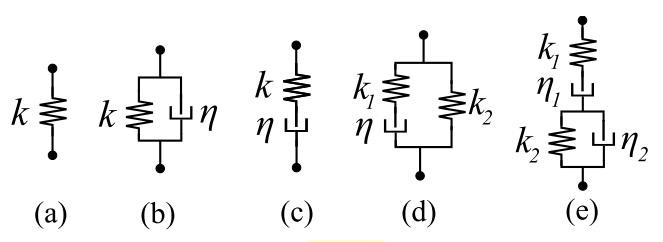
\includegraphics[width=0.6\textwidth]{HookeViscoelasticModels.PNG}
    \caption{Hooke's Law and linear viscoelastic models: (a) Hooke's Law (b) Kelvin-Voigt, (c) Maxwell, (d) Standard Linear Solid, and (e) Burger. The parameters $k$ and $\eta$ represent the spring stiffness and the dashpot viscous constant, respectively \cite{austin2015control}. }
    \label{fig:LinearViscoelasticModels}
\end{figure}

In line with the mentioned approach of relying on the controller to compensate the limitations of simple models, the work performed by Austin et al. modifies the viscoelastic Standard Linear Solid (SLS) model by implementing a piecewise linearization (PL) \cite{austin2015control}. The authors chose this model instead of the more complete, hence more complex, Burger model to keep the modelling process as simple as possible. The implementation of the PL method allowed the SLS model to account for the nonlinear properties of the material stress response in proportion to the applied strain. Due to this, the developed model is called the Standard Linear Solid model with Strain-Dependent Stiffness (Std. Lin. SDS). Unfortunately, the developed model was still unable to account for the material hysteresis, and, due to hardware limitations, the velocity-dependent stiffness effects were not validated. Nonetheless, experimental tests validated the changes on the material stiffness depending on the velocity of the applied deformation.

The PL method have proven to be a successful way to improve the prediction ability of traditional LVMs. Although it still has some limitations. The latter is addressed in this chapter by implementing the PL method in a more complex member of the LVMs, the Wiechert model. This is described in detail in \Cref{sec:wiechert}.

\section{The Piecewise Linearization Method} \label{sec:wiechert}

The SLS model is frequently used when modelling viscoelastic materials, mainly due to its fairly simple mathematical model and its ability to account for creep and stress relaxation of the material (time-dependent properties). The SLS model can be viewed as a Maxwell model (also known as Maxwell branch) with an extra spring connected in parallel. The simplicity of the SLS model is also its main limitation. 
Viscoelastic materials are known to have more than one relaxation time, i.e. more than one Maxwell branch. In the linear viscoelastic models, the relaxation time depends on the viscous elements, i.e. dashpots. The Wiechert model, which is essentially a SLS model with $j$ Maxwell branches, is able to account for $j$ relaxation times and is illustrated in \Cref{fig:wiechert}. The time-dependent behavior of any viscoelastic material can be fully described by this model, given enough numbers of elements. However, the complexity of the model increases in proportion to the number of extra branches. Mathematically, each extra branch increases the derivative order of the model since more equations are required to account for the extra variables \cite{tirella2014strain,roylance2001engineering}.

\begin{figure}[hbt!]
	\centering
    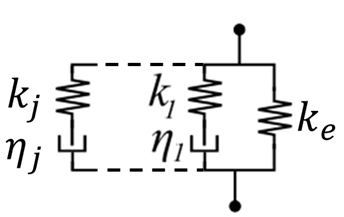
\includegraphics[width=0.3\textwidth]{WiechertModel.png}
    \caption{Wiechert Model. The components $k_1$, $\eta_1$, and the equilibrium spring $k_e$, together represents the SLS model. The components $k_j$, and $\eta_j$ represents the Maxwell Branch. The Wiechert model can contain as many branches as required, this is symbolised by the subscript $j$. }
    \label{fig:wiechert}
\end{figure}

As previously described in \Cref{sec:mechprop}, in addition to time-dependent and history-dependent properties, elastomers also have a nonlinear stress response. This can be partially described by the LVMs. The relaxation time constant of the dashpots in these models describes the nonlinear and time-dependent stress response of the material. Nonetheless, LVMs are not able to account for the strain-dependent response of materials. The latter can be addressed by the PL method as described in \cite{austin2015control}.

The spring in parallel with the other elements, in both the SLS model and the Wiechert model, is known as the equilibrium spring, and its stiffness $k_e$, is assumed constant. In reality, the stiffness $k_e$ of most elastomers is strain-dependent. Early attempts of modelling a strain-dependent stress response in viscoelastic materials are described by Schepelmann et al. in \cite{schepelmann2014compact}, where the stress-strain curve of a nonlinear rubber spring is approximated with an exponential model. In subsequent works, Austin et al. describe a piecewise linear regression fitted to the stress-strain curve of a material, in combination with the SLS model \cite{austin2015control}. 

The slope of the stress-strain curve represents the material's Young Modulus which is proportional to the material stiffness. During a tensile strength test the material is deformed at a constant rate, i.e. $\dot{\varepsilon}$ is constant. The stress response of a viscous element is proportional to the strain rate $\dot{\varepsilon}$. Therefore, it can be safely assume that the observed nonlinear stress response  on the stress-strain curve is solely caused by changes in the equilibrium spring stiffness $k_e$.

Using the PL method, the nonlinear behavior of the equilibrium spring is approximated by considering it as several springs in parallel which ``engage'' in sequence as the material strain increases. This is modeled by a summation of Heaviside functions centered in the desired strain in which each of the mentioned springs ``engage'' and contributes with the total stress response of the material. In other words, the stress-strain curve of the material is segmented in several sections which relates a single stiffness to a range of strains. This is illustrated in \Cref{fig:PLmethod}.

\begin{figure}[htb!]
	\centering
    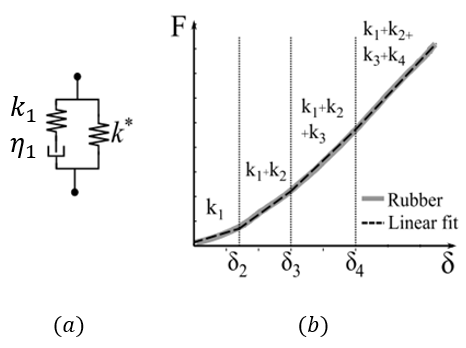
\includegraphics[width=0.6\textwidth]{PLmethod.png}
    \caption{(a) Standard Linearized Solid model with Strain-Dependent Stiffness. (b) Piecewise linearization method applied to the slope of the material load-displacement curve. This is analogous to many parallel springs which contribute to the material response depending on the material strain \cite{austin2015control}}.
    \label{fig:PLmethod}
\end{figure}

\section{Model fitting} \label{sec:Modelfit}

The mathematical expression for the SLS model and the Wiechert model can be simplified when considering a constant strain input (stress relaxation test). This simplification allows these models to be fitted into the stress relaxation curve and to approximate the parameters of interest, $k$ and $\eta$ \cite{roylance2001engineering}. The mathematical expression for the Wiechert model under a constant strain input is given by:

\begin{equation}
\label{eq1}
\sigma (t) = \left( k_e +  \sum_{j} k_j e^{-t/\tau_j} \right)  \varepsilon_o
\end{equation}

\noindent where $\sigma$ is the stress at a given time, $k_e$ is the equilibrium spring stiffness and $\varepsilon_o$ is the initial strain. For the summation, $\tau_j=\eta_j/k_j$ is the relaxation time constant, $k_j$ and $\eta_j$ are the spring stiffness and viscous constant of the elements in the $j^{th}$ Maxwell branch, respectively. For the specific case when $j = 1$, the resulting equation describes the SLS model under a constant strain input, which is as follows:

\begin{equation}
\label{eq11}
\sigma(t) = \left( k_e +  k_1 e^{-t/\tau} \right)  \varepsilon_o
\end{equation}


In \Cref{eq11}, the three main parameters of the SLS model. i.e. the equilibrium spring stiffness $k_e$, the dashpot viscous constant $\eta = \tau k_1$, and the spring stiffness in the Maxwell branch $k_1$, can be obtained from the stress relaxation curve by analyzing three significant points: $t=0$, $t=\tau$, and $t=\infty$, as illustrated in \Cref{fig:stressTimeCurve}. Due to the decaying exponential nature of this curve, the time constant $\tau$ can be related to the point in time $t$ where the stress has decayed to approximately 36.8\% of its initial value $\sigma_o$. The longer the duration of the test, the better the approximation of $k_e$.

\begin{figure}[htb!]
	\centering
    
\includegraphics[width=0.5\textwidth]{StressTimeCurve.png}
    \caption{SLS model fitted to a typical stress relaxation curve of a viscoelastic material. The parameters $k_e$, $k_1$ and $\eta$ can be obtained by analyzing three points in the curve: $t=0$, $t=\tau$, and $t=\infty$. The variable $\tau$ is the time constant of the exponential decaying curve.}
    \label{fig:stressTimeCurve}
\end{figure}

The process to extract the parameters of the Wiechert model is more complicated due to its extra Maxwell branches, i.e. there are more than three points in time to be analyzed. These points can be selected using a collocation technique \cite{roylance2001engineering,machiraju2006viscoelastic}. In the reviewed literature, the points of interest are linearly scattered throughout the whole duration of the stress relaxation curve. Nevertheless, the decaying exponential term in \Cref{eq1} is better approximated by selecting the points of interest using a logarithmic scale. This is possible with the MATLAB function \texttt{logspace} which spreads evenly the desired number of points between the allowable decades. 
This is better described with the following example. A Wiechert model with six branches, $j=6$, is to be fitted into a stress relaxation curve with four decades of duration ($t=10^4$ seconds). In total it would be required seven points in time, one for each branch and one for $t=0$. These points are spread as evenly as possible, using the total duration of the test, by the function \texttt{logspace}. The point $t=0$ is required for a correction described in the following paragraph. 

Similar to the process illustrated in \Cref{fig:stressTimeCurve}, each point in time represents a time constant $\tau_j$ for which there is a known stress $\sigma_j$ from the experimental data. This can be rearranged into an equation system of $j$ equations with $k_j$ as the unknown variable as described in \cite{machiraju2006viscoelastic}. 

%Maybe bring the system of equations here?

Prior to this step, $k_e$ can be obtained using the equation for $\sigma(\infty)=\varepsilon_o k_e$, as illustrated in \Cref{fig:stressTimeCurve}. Subsequently, the Wiechert model in \Cref{eq1} can be completely described by solving the mentioned system of equations. Finally, after obtaining all the $k_j$, the value of $k_1$ is corrected, as described in \cite{roylance2001engineering}, by analyzing the point in time $t=0$.

The previous process allows the Wiechert model equation to be fitted into the stress relaxation curve for a defined number of branches $j$. However, to obtain the optimal number of branches for each material, an iterative algorithm to find the smallest root mean square error (RMSE) between the Wiechert model response and the experimental data after testing different number of branches in the range of $j=[1,10]$ is implemented. The obtained optimal number of branches for each material varied between the range $j=[5,8]$. A higher number of branches has a meaningless improvement on the RMSE. Furthermore, beyond the number of branches $j=20$ the Wiechert model response shows an oscillatory behavior, hence a higher RMSE. Having obtained the parameters of interest for the SLS and the Wiechert model, their stress response under a constant strain is compared against the experimental data in \Cref{fig:StressRelFit}.

\Cref{fig:StressRelFit} highlights the better accuracy delivered by the extra Maxwell branches in the Wiechert model in comparison to the simpler SLS model. As previously mentioned, \Cref{eq1} is a simplification helpful to approximate the parameters of both models but it is only applicable when the strain input is constant. The mathematical expression for the Wiechert model which describes the stress response under an unknown strain input, also called the constitutive equation can be found in \cite{roylance2001engineering}, in its Laplace. 
As previously mentioned, the Wichert model is an extension of the SLS model. Hence, when making $j=1$, the constitutive equation of the SLS model can be obtained, i.e. for an unkown strain input, and is presented as follows:

\begin{figure}[htb!]
	\centering
    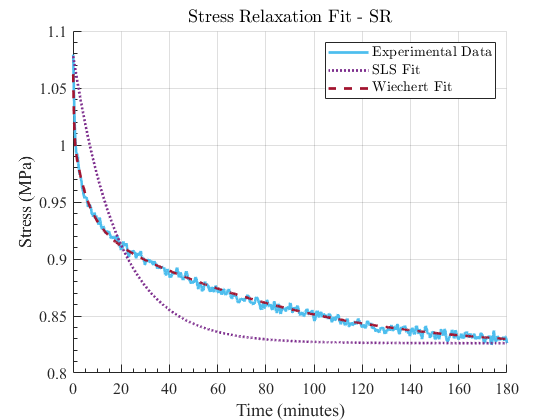
\includegraphics[width=0.8\textwidth]{SRelFit.png}
    \caption{Obtained fit from the Standard Linear Solid (SLS) and Wiechert model on the stress relaxation curve of the Silicone Rubber material. The obtained optimal number of branches of the Wiechert model fit is $j=8$.}
    \label{fig:StressRelFit}
\end{figure}

\begin{equation}
\label{eq3}
\dot{\sigma} + \frac{\sigma}{\tau_1} =  (k_e + k_1)\dot{\varepsilon} + \frac{k_e\varepsilon}{\tau_1}
\end{equation}

\noindent where $\varepsilon$, $\dot{\varepsilon}$, and $\dot{\sigma}$ are the strain, the strain rate and the stress rate, respectively (for the detailed procedure refer to \cite{roylance2001engineering}). Notice that the previous procedure will yield into a higher derivative order equation when applied to the Wiechert model due to its extra branches. A higher number of branches will increase the model accuracy at the cost of increasing its mathematical complexity. The constitutive equation of a Wiechert model with $j$ branches would result in a $j$ order differential equation similar to \Cref{eq3}. The aim of this chapter is to apply the PL method to the Wiechert model and evaluate its performance. Therefore, dealing with differential equations is out of the scope. Nonetheless, the Wiechert model can be evaluated by transforming it into a finite-differences equation, as explained in \cite{roylance2001engineering}, yielding the following equation:

\begin{equation}
    \label{eq4}
    \sigma^t = k_e\varepsilon^t + \sum_j \frac{k_j(\varepsilon^t - \varepsilon^{t-1}) + \sigma_j^{t-1}}{ \left( 1+\dfrac{\Delta t}{\tau_j} \right) }
\end{equation}

\noindent where the superscript $t-1$ and $t$ refers to values before and after a small time step $\Delta t$ have passed. Once again, making $j=1$ in \Cref{eq4} yields the finite difference version of the SLS model. The response of the two viscoelastic models of interest will be compared against the experimental data from the tensile strength test.

The next step of the fitting process is focused on the tensile strength test. In this test, the strain rate is constant, hence the resulting stress for both models (\Cref{fig:LinearViscoelasticModels}) is dependent on both the equilibrium spring and the Maxwell branches. At this stage of the model fitting process, the parameters of the Maxwell branches in both models are known and their stress response can be calculated. The stress response of the equilibrium spring, $k_e$, can be isolated by subtracting the stress response of the Maxwell branches to the stress measured in the tensile strength test. 

After isolating the stress response of $k_e$, the final step in the fitting process is to implement the PL to both models and compare their response against the experimental data. Firstly, the stress-strain curve from the tensile strength test is divided into $n$ segments. As previously explained, $k_e$ is considered as a group of parallel springs which ``engage'' as the strain increases. This means, each subsequent stiffness is a combination of the ones found in previous segments of the stress-strain curve (\Cref{fig:PLmethod}).  Lastly, a linear regression is applied on the stress-strain curve for the desired $n$ strain segments to find the slope of the curve. This slope represents the stiffness of the equilibrium spring in each segment. By combining the $n$ obtained stiffness, the stress response of the strain-dependent stiffness $k_i^*$ is defined as follows:

\begin{equation}
\label{eq5}
\sigma^{*^t} = \sum_i^n k_i^* H_{\varepsilon - \varepsilon_i}(\varepsilon^t - \varepsilon_i)
%\sigma^* = \sum_i^n k_i^* H_{\varepsilon - \varepsilon_i}(\varepsilon - \varepsilon_i)
\end{equation}

\noindent where $n$ is the desired number of strain intervals to fit, $\varepsilon_i$ represents the strain value at which the $i^{th}$ spring starts contributing to the stress response, the $H_{\varepsilon - \varepsilon_i}$ is the Heaviside or unitary step function centered at $\varepsilon_i$, i.e. the function output goes from 0 to 1 when $\varepsilon - \varepsilon_i = 0$. By substituting \Cref{eq5} into \Cref{eq3}, the Standard Linear Solid model with Strain-Dependent Stiffness is obtained \cite{austin2015control}.

The LVMs describe a nonlinear relationship between the applied strain and the resulting stress in a material. However, they only account for a linear stress response of the equilibrium spring. In reality, the relocation of internal molecular chains causes viscoelastic materials to exhibit a nonlinear and strain-dependent stress response. This can be solved by implementing a PL into \Cref{eq4}. The equilibrium spring stiffness $k_e$ is replaced by the strain-dependent stiffness $k_i^*$, yielding the linearized Wiechert model (PL-Wiechert) in \Cref{eq6}. Subsequently, the Std. Lin. SDS model, found in \cite{austin2015control}, is transformed into a finite difference equation, yielding the PL-SLS model described in \Cref{eq7}.

\begin{equation}
\label{eq6}
\sigma^t = \sigma^*{^t} + \sum_j \frac{k_j (\varepsilon^t-\varepsilon^{t-1}) + \sigma_j^{t-1}}{\left( 1 + \dfrac{\Delta t}{\tau_j}\right) }
\end{equation}

\begin{equation}
\label{eq7}
\sigma^t = \sigma^*{^t} + \frac{k_1(\varepsilon^t - \varepsilon^{t-1}) + \sigma_m^{t-1}}{ \left( 1+\dfrac{\Delta t}{\tau_1} \right) }
%\sigma^ t = \frac{1}{\left( 1+\dfrac{\Delta t} {\tau} \right) } \left[  \frac{\Delta t}{\tau} \sigma^* + (\sigma^* + k_1) (\epsilon^t-\epsilon^{t-1}) + \sigma^{t-1} \right]  
\end{equation}

In this chapter, the linearized SLS model in \Cref{eq7} is labeled as the piecewise linearized SLS (PL-SLS) model, differentiating it from the Std. Lin. SDS model documented in \cite{austin2015control} due to the different fitting process performed, e.g. removing the stress response of Maxwell branches. The experimental data from the stress relaxation test was used to obtain the parameters in the Maxwell branches of both models. Lastly, the required number of branches was different per material, ranging from $j=5$ to $j=8$. Lastly, the process of fitting the piecewise linearization method to the SLS and the Wiechert model to create the PL-SLS and the PL-Wiechert model is described in \Cref{fig:FCFittingProcess}.

\begin{figure}[H]
	\centering
	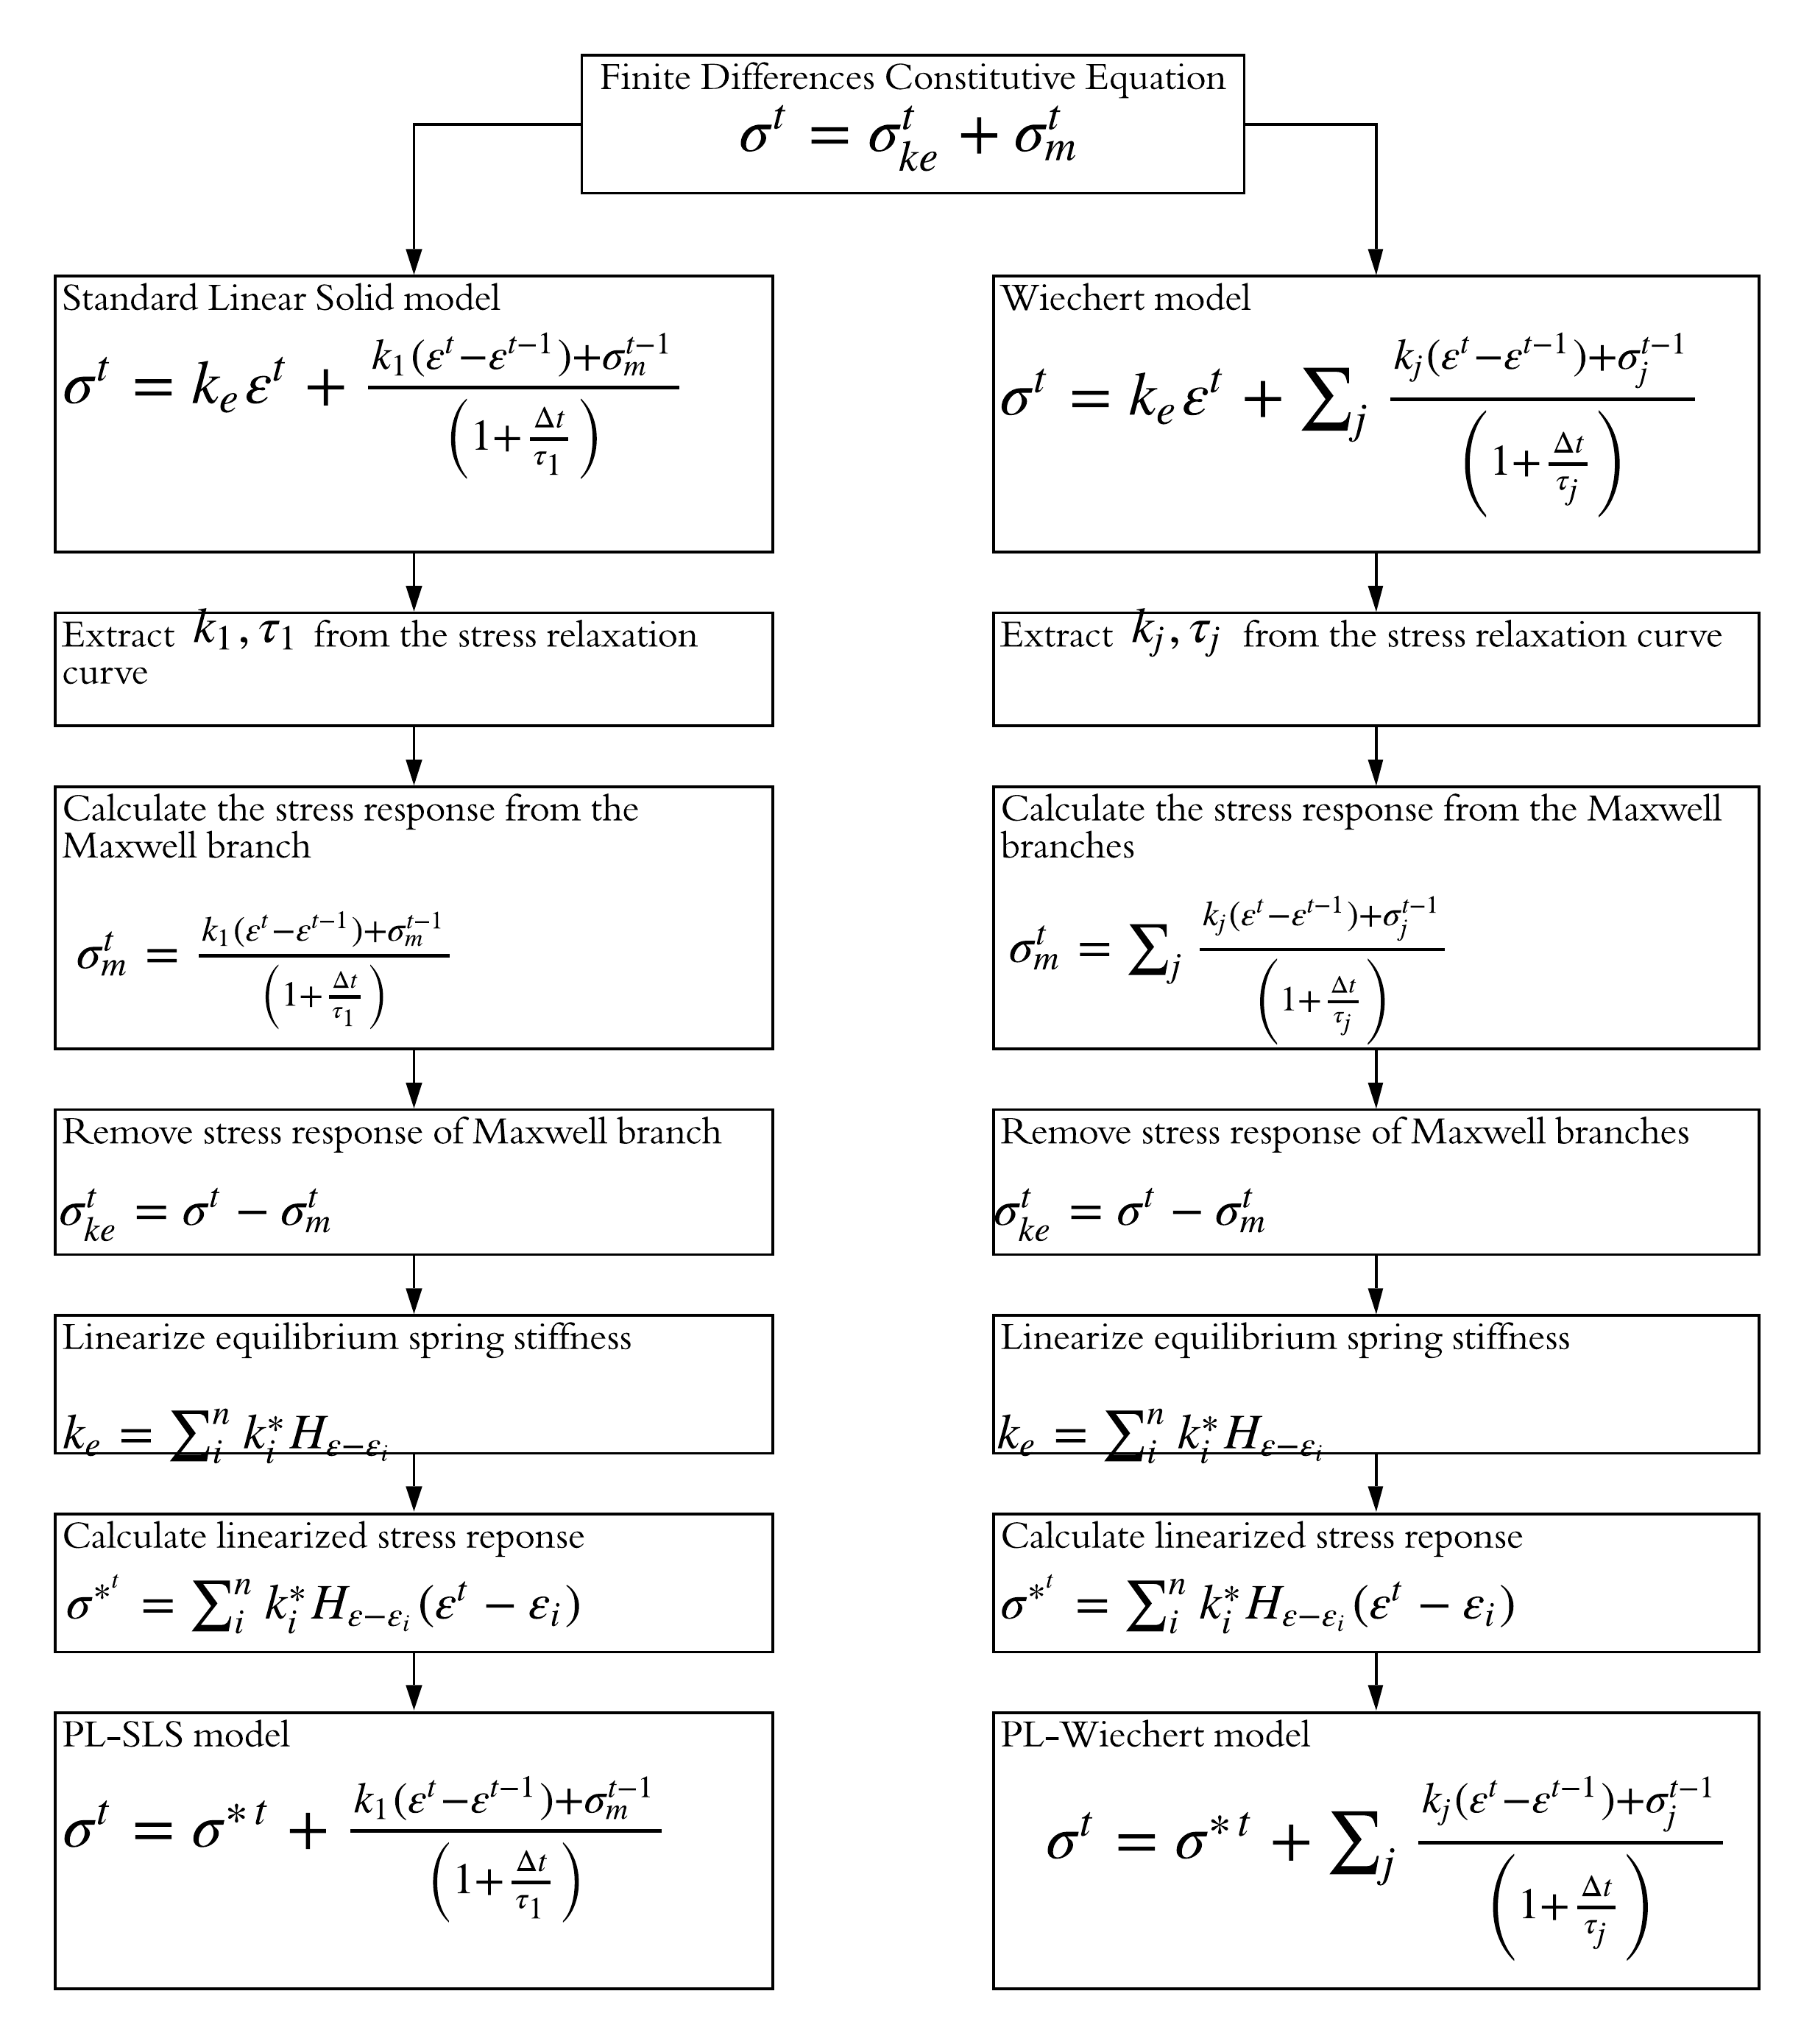
\includegraphics[width=\textwidth]{FitProcessPLMethod.png}
	\caption{ Description of the piecewise linearization method implemented in this work.}
	\label{fig:FCFittingProcess}
\end{figure}

\newpage

\section{Findings}

The following section describes the findings obtained from three individual analyses about the PL method performance and capabilities. The latter is organized in three subsections. \Cref{SegmentAnalysis} is focused on analyzing the trade-off between the number of strain segments fitted to the stress-strain curve, i.e. complexity, and the achieved accuracy, when being applied to the PL-SLS model and the PL-Wiechert model. \Cref{ModelfitAnalysis} is focused on analyzing the accuracy of the PL-SLS model and the PL-Wiechert model in terms on the achieved normalized mean square error (NRMSE). Lastly, \Cref{VelocityAnalysis} is focused on analyzing the capabilities of both models to account for the velocity dependency of the materials stress response. In other words, the generalization capabilities of both models are assessed.

The stress-strain curves from the materials studied in this section are from the tensile strength test with 500 mm/min strain rate. With the exception of the SR material, for which the stress-strain curve for a strain rate of 50 mm/min is used. The available data for each soft material is described in \Cref{tbl:tensile_tests}.

\subsection{Analysis of the optimal number of strain segments} \label{SegmentAnalysis}

The amount of strain segments and their proper collocation have an impact on the PL method accuracy. In the work presented by Austin et al. there is no explanation about the criteria used to select the strain segments. Nonetheless, the implementation of a linear collocation approach is suggested \cite{austin2015control}. 

In here, the variation of the slope in the stress-strain curve is proposed as a selection criteria for obtaining the right number of strain segments to fit to the stress-strain curve of the materials. Hence, an algorithm is developed to automatically collocate a new strain segment when the curve's slope exhibits a variation greater than a proposed tolerance value. In the optimization process the testing of different tolerance values in the range of 10 to 100 \% is performed. This process is described in \Cref{fig:FCsegments}. 

\begin{figure}[H]
	\centering
	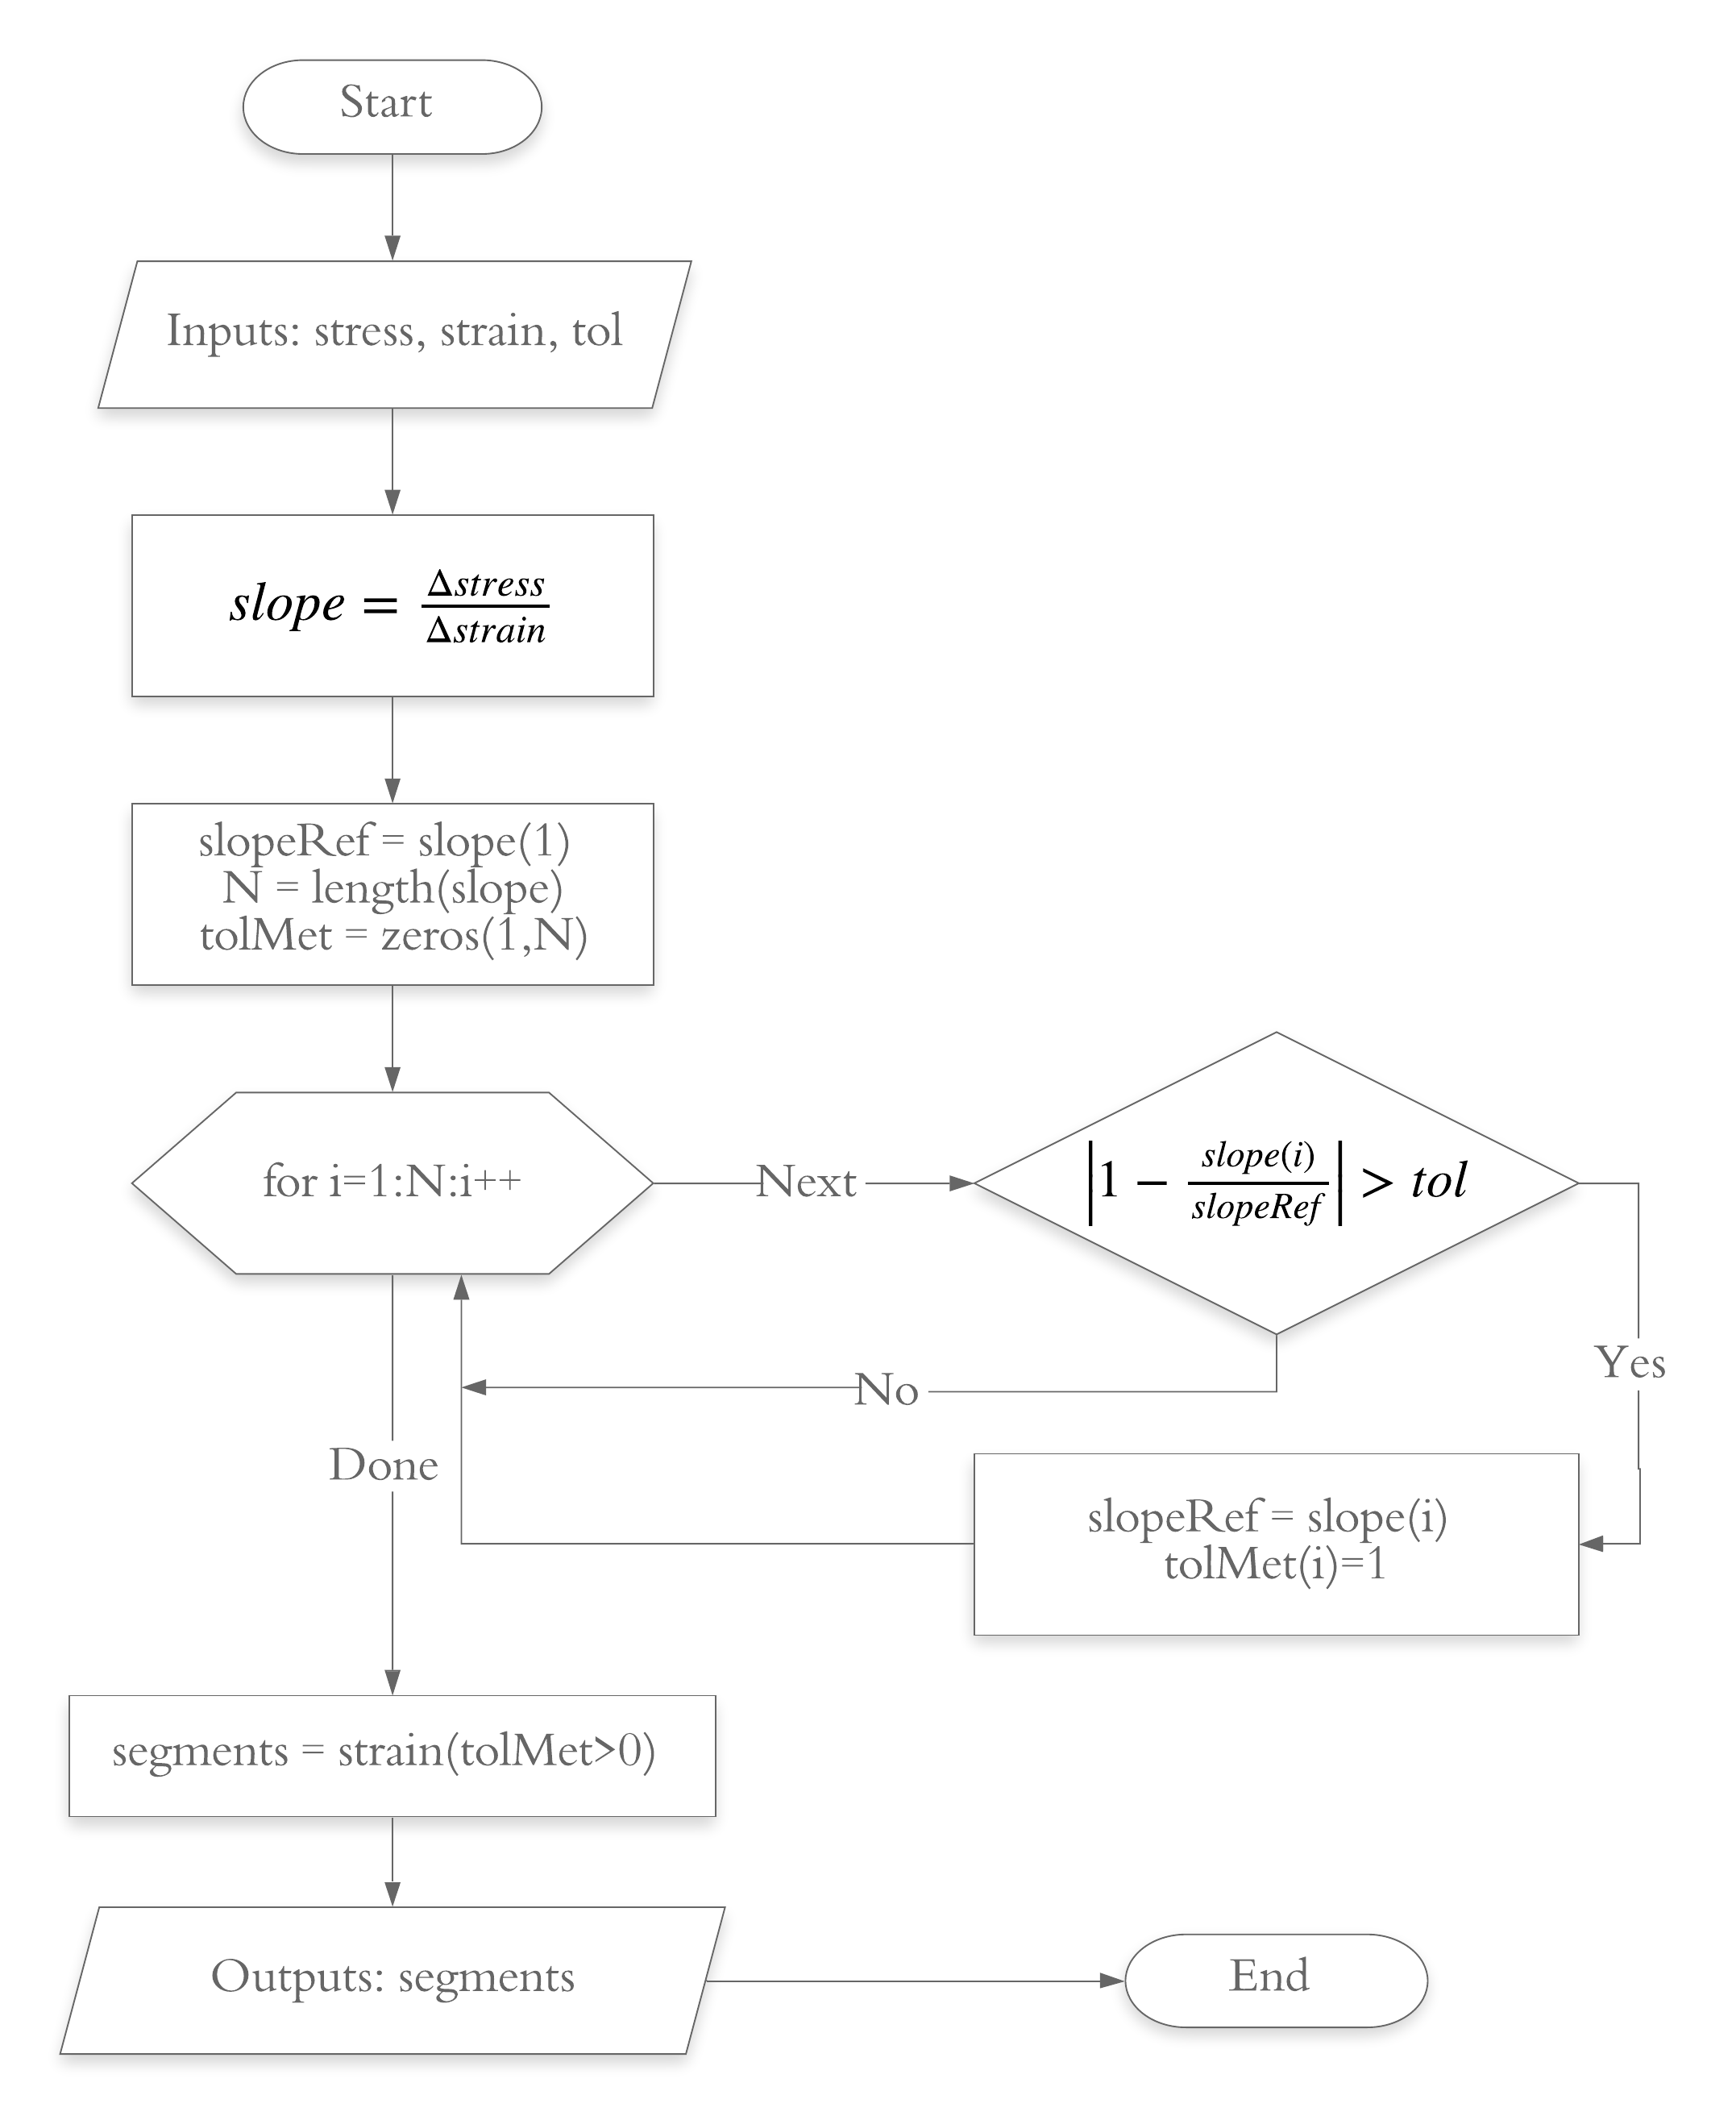
\includegraphics[width=\textwidth]{StrainSegmentsOptimization.png}
	\caption{ Algorithm for obtaining the right number of strain segments to be fitted based on the variation of the stress-strain curve slope.}
	\label{fig:FCsegments}
\end{figure}

The slope is calculated by numerical differentiation of the stress-strain curve. Then, the first calculated value of the slope is used as reference to monitor the variation of the slope along the stress-strain curve. When the variation is greater than the defined tolerance two things happen: a new strain segment is created, and the slope at this point becomes the new slope reference. This process is repeated until the complete stress-strain curve scanned.

The proposed tolerance criteria establishes a proportional relationship between the nonlinearity of the stress-strain curve and the complexity of the piecewise linearization process. In other words, highly nonlinear soft materials will require more strain segments to be collocated. In a similar way, the tolerance criteria is inversely proportional to the obtained number of strain segments. In other words, the smaller the tolerance the larger the number of strain segments.

The performance of the PL method can be analyzed with the optimization process described. Specifically, the relationship between the complexity and accuracy of the PL method. The complexity of the PL method is measured in terms of the number of strain segments fitted to the stress-strain curve. Whereas, the accuracy of the PL method is measured in terms of the normalized root mean square error (RMSE) \cite{bergstrom2015mechanics}, described as follows:

\begin{equation}
    \mathrm{NRMSE} = \sqrt{  \frac{\langle (\sigma^{pred} - \sigma^{exp})^2 \rangle}{\langle {\sigma^{exp}}^2 \rangle} }
\label{eq2}
\end{equation}

\noindent where the  $\langle ... \rangle$ represents the arithmetic mean, $\sigma^{pred}$ and $\sigma^{exp}$ represent the predicted and experimental values of the stress response of the material, respectively. The results of the optimization process are illustrated in \Cref{fig:SegmentsEPR_FR,fig:SegmentsNR_NatR,fig:SegmentsPR_SR,fig:SegmentsNat100R}. In these figures, the inversely proportional relationship between the number of strain segments and the tolerance is demonstrated. In other words, the smaller the tolerance value the greater the number of strain segments. In general, the relationship between these two parameters is inversely exponential for both the PL-SLS model and the Wiechert model. This is consistent with all but one of the studied soft materials, the SR material. In this case, the relationship between the tolerance value and the number of strain segments, for both models, is more linear than exponential. There is in fact a complex relationship between the number of strain segments, the tolerance criteria, the achieved accuracy and the model used.

\newpage

\begin{figure}[H]
	\centering
	\begin{subfigure}[b]{0.9\textwidth}
		\centering
		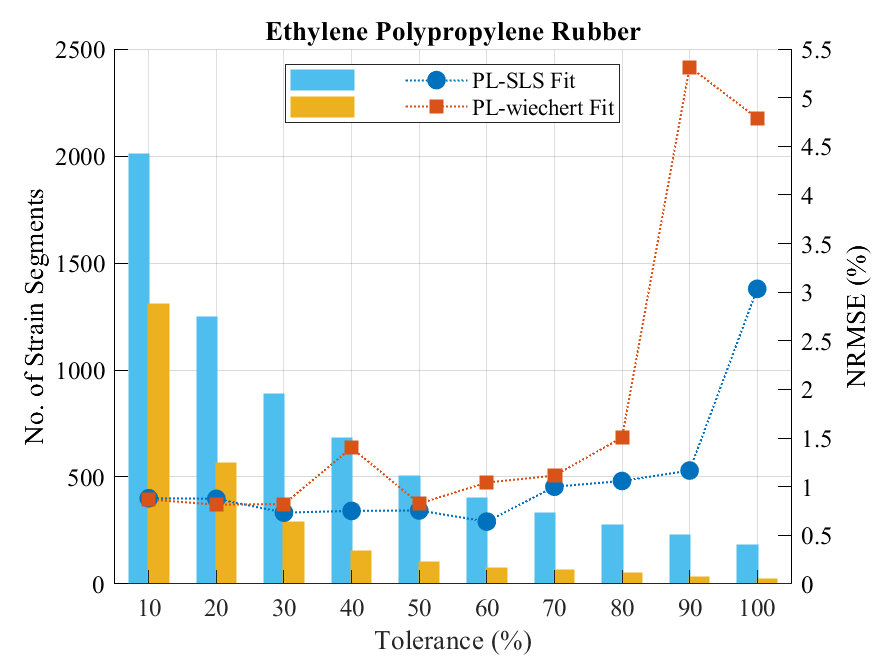
\includegraphics[width=\textwidth]{EPR_PLMethodFit.png}
		\caption{}
		\label{fig:SegmentsEPR}
	\end{subfigure}
	\begin{subfigure}[b]{0.9\textwidth}
		\centering
		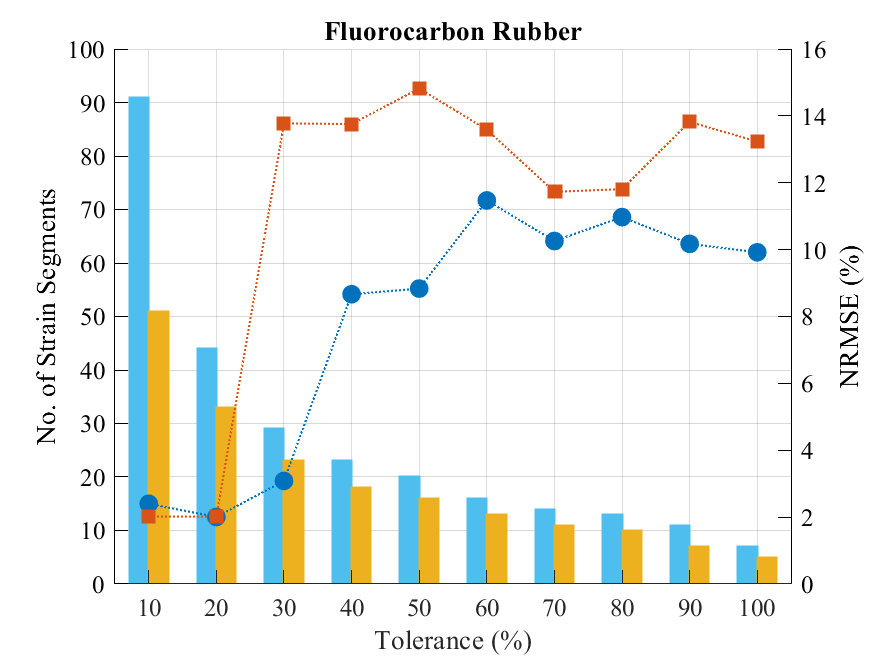
\includegraphics[width=\textwidth]{FR_PLMethodFit.png}
		\caption{}
		\label{fig:SegmentsFR}
	\end{subfigure}
	\caption{Impact of the proposed tolerance criteria on the relationship between the number of strain segments and the achievable accuracy of the PL method. (a) EPR material (b) FR material.}
	\label{fig:SegmentsEPR_FR}
\end{figure}

\begin{figure}[H]
	\centering
	\begin{subfigure}[b]{0.9\textwidth}
		\centering
		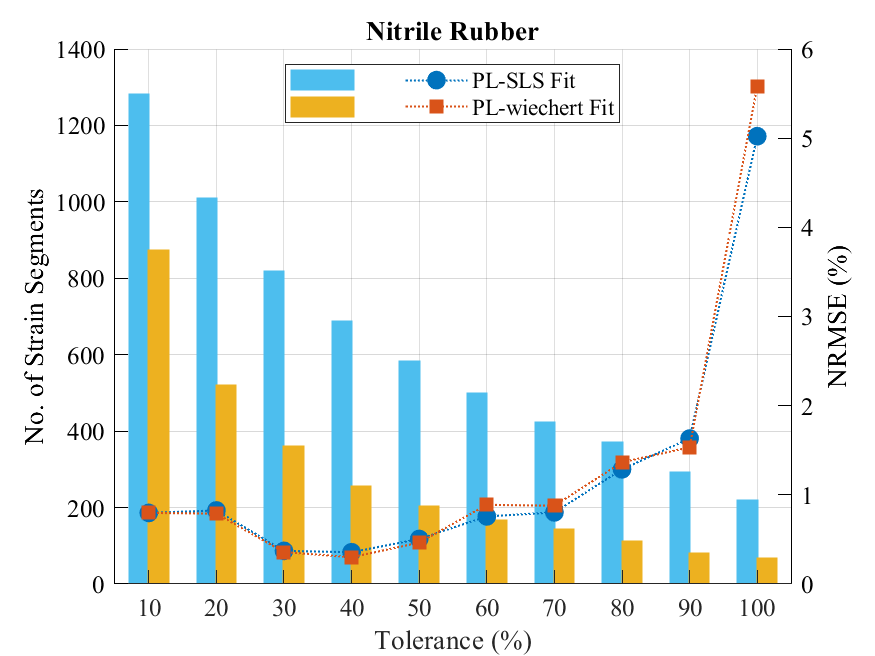
\includegraphics[width=\textwidth]{NR_PLMethodFit.png}
		\caption{}
		\label{fig:SegmentsNR}
	\end{subfigure}
	\begin{subfigure}[b]{0.9\textwidth}
		\centering
		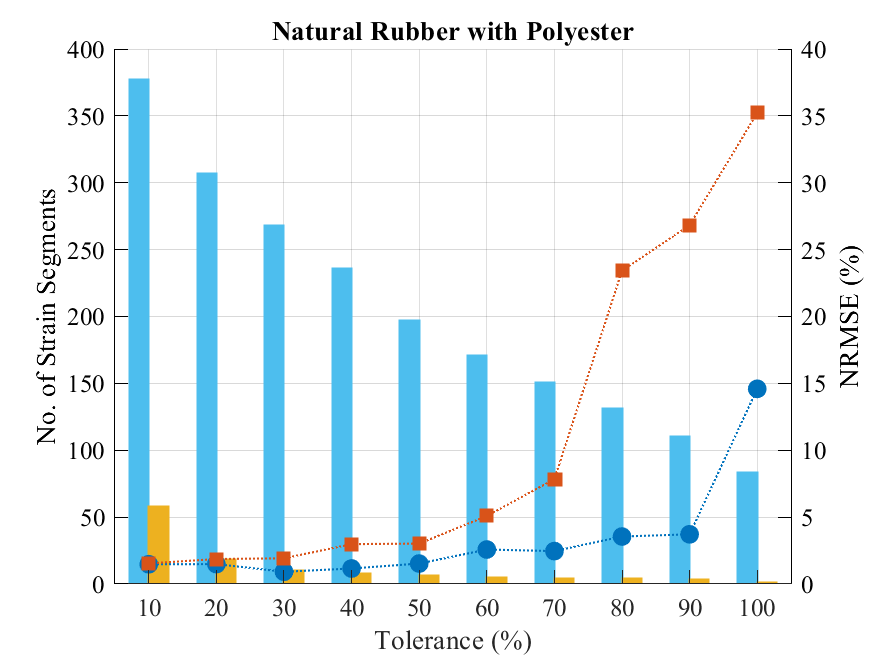
\includegraphics[width=\textwidth]{NatR_PLMethodFit.png}
		\caption{}
		\label{fig:SegmentsNatR}
	\end{subfigure}
	\caption{Impact of the proposed tolerance criteria on the relationship between the number of strain segments and the achievable accuracy of the PL method. (a) NR material (b) NatPolR material.}
	\label{fig:SegmentsNR_NatR}
\end{figure}

\begin{figure}[H]
	\centering
	\begin{subfigure}[b]{0.9\textwidth}
		\centering
		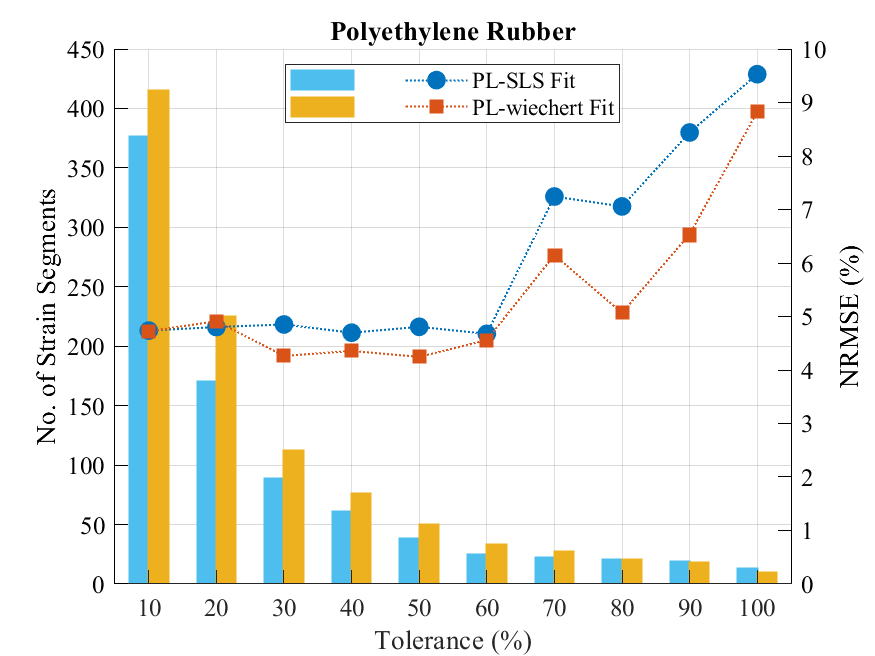
\includegraphics[width=\textwidth]{PR_PLMethodFit.png}
		\caption{}
		\label{fig:SegmentsPR}
	\end{subfigure}
	\begin{subfigure}[b]{0.9\textwidth}
		\centering
		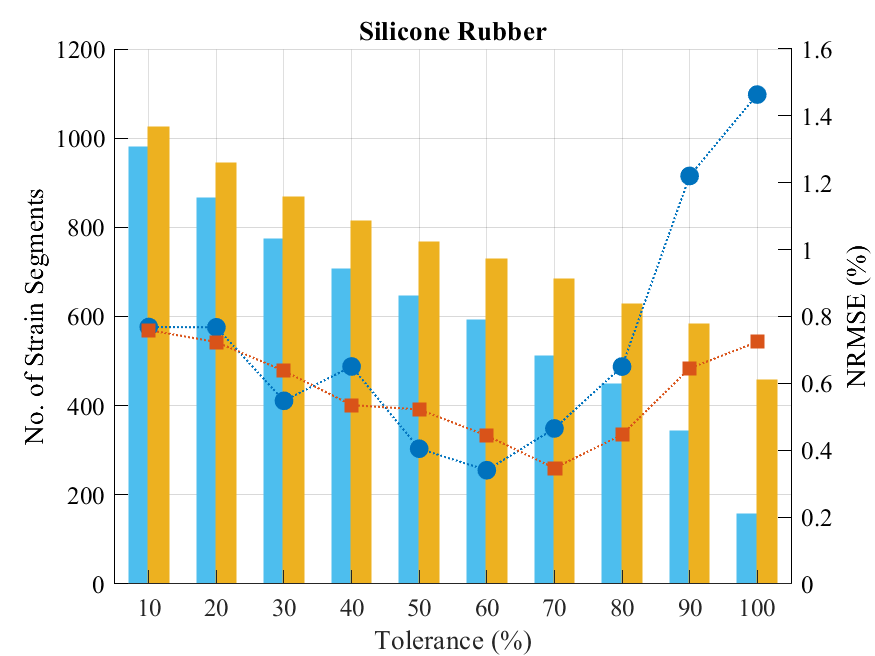
\includegraphics[width=\textwidth]{SR_PLMethodFit.png}
		\caption{}
		\label{fig:SegmentsSR}
	\end{subfigure}
	\caption{Impact of the proposed tolerance criteria on the relationship between the number of strain segments and the achievable accuracy of the PL method. (a) PR material (b) SR material.}
	\label{fig:SegmentsPR_SR}
\end{figure}

\begin{figure}[H]
	\centering
	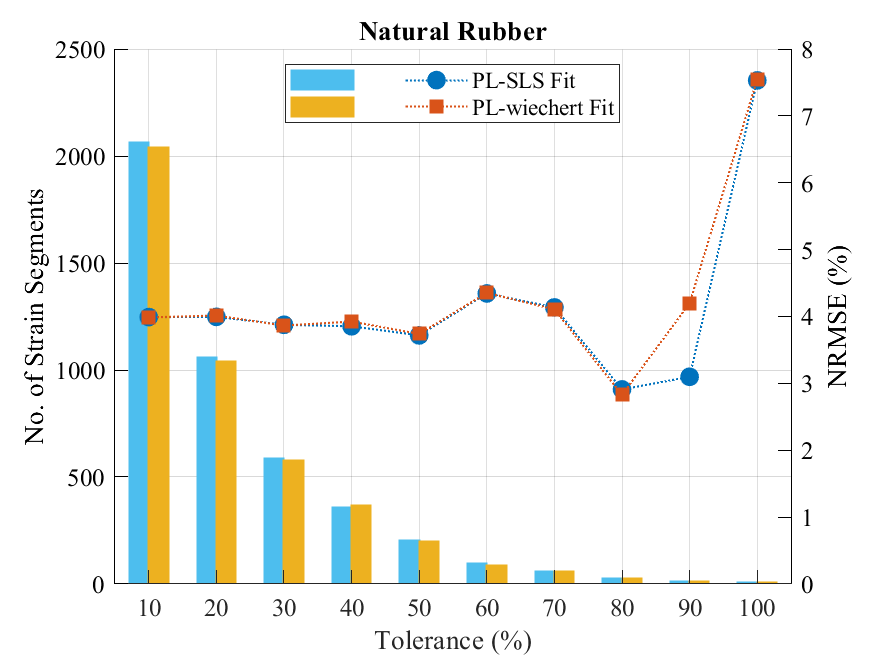
\includegraphics[width=0.9\textwidth]{Nat100R_PLMethodFit.png}
	\caption{Impact of the proposed tolerance criteria on the relationship between the number of strain segments and the achievable accuracy of the PL method. NatR material}
	\label{fig:SegmentsNat100R}
\end{figure}

In general, there is no substantial difference on the best obtained accuracy of both models. The main difference between the models is the number of strain segments required to achieve this accuracy. In most of the cases, the PL-Wiechert model requires fewer strain segments than the PL-SLS model. This is the case for the EPR, FR, NR, NatPolR and NatR materials (\Cref{fig:SegmentsEPR_FR,fig:SegmentsNR_NatR,fig:SegmentsNat100R}). In these cases, the benefit of isolating the stress response of the equilibrium spring stiffness $k_e$ by subtracting the stress response of the Maxwell branches from the stress-strain curve of the materials is appreciated. The latter essentially split the stress response of the material in two parts: the time dependent stress response and the nonlinear strain-dependent stress response. The PL-Wiechert model, which has a larger number of Maxwell branches, is expected to describe the time dependent stress response more accurately than the PL-SLS model. This allows the PL method to be more effective in modelling the nonlinear strain-dependent stress response. The effectiveness of the latter process is dependent on the properties of the soft material in turn. The materials with dominant viscoelastic properties are benefited the most when using the PL-Wiechert method. In fact, it is possible to categorize the studied soft materials into: highly elastic (\Cref{fig:SegmentsPR_SR,fig:SegmentsNat100R}), viscoelastic (\Cref{fig:SegmentsFR,fig:SegmentsNR}), and highly viscous (\Cref{fig:SegmentsEPR,fig:SegmentsNatR}), by analyzing the difference on the required number of strain segments between the PL-SLS model and the PL-Wiechert model.

Another important finding is the speed in which both models converge to the smallest NRMSE value. In this scenario, the PL-SLS model is faster than the PL-Wiechert model. In general, it is safe to assume that the smallest tolerance criteria does not always yield in the best accuracy for both models. In other words, there is a tolerance value which delivers the best accuracy for each individual model. The latter is analyzed in the following section. In summary, the analysis performed in this section describes the relationship between the complexity of the PL method and its accuracy when being applied to the LVMs. 


\subsection{Analysis of model fit accuracy} \label{ModelfitAnalysis}

In this section, the goodness of fit of both developed models is analyzed. In general, both the PL-SLS model and the PL-Wiechert model converge to very similar NRMSE values when enough number of strain segments are used. The main difference between the models is the number of strain segments required for convergence. In most cases, the PL-SLS model requires fewer strain segments to converge than the PL-Wiechert model. This is illustrated in the previous section \Cref{fig:SegmentsEPR_FR,fig:SegmentsNR_NatR,fig:SegmentsPR_SR,fig:SegmentsNat100R}. In this section, the best case performance of both models is analyzed. The latter aims to test the hypothesis that a better model can be developed by implementing the PL method to more complex LVMs, i.e. the Wichert model. The latter can be tested by calculating the increment or decrement achieved by the PL-Wiechert model with respect to the PL-SLS model, for both the accuracy and number of strain segments, as follows:

\begin{equation}
	\Delta Accuracy = 100\left(1 - \frac{NRMSE_{Wiechert}}{NMRSE_{SLS}} \right)
\end{equation}

\begin{equation}
	\Delta Complexity = 100\left( \frac{Segments_{Wiechert}}{Segments_{SLS}} - 1 \right)
\end{equation}

\noindent where $\Delta Accuracy > 0$, and $\Delta Complexity < 0$, represents the improvement achieved by the PL-Wiechert model with respect to the PL-SLS model. In \Cref{tbl:PLModelsPerformance}, the best performance case for both models is compiled. In here, the performance of the PL-Wiechert model is compared against the performance of the PL-SLS model.

\begin{table*}[htbp!]
	\centering
	\caption{Best accuracy of the PL-SLS (1) and the PL-Wiechert (2) models.}
	\label{tbl:PLModelsPerformance}
	\begin{tabular}{llccccccc} \toprule
		Model 					& Parameters 		& EPR	& FR & NatPolR & NR & PR & SR & NatR \\
		\hline
		\multirow{3}{*}{1}  & NMRSE (\%)		& 0.64	& 2 & 0.91 & 0.35 & 4.67 & 0.34 & 2.90 \\
								& Segments		& 400	& 44 & 268 & 686 & 25 & 592 & 27 \\
								& Tolerance (\%)	& 60	& 20 & 30 & 40 & 60 & 60 & 80 \\
		\hline 
		\multirow{6}{*}{2}  & NMRSE (\%)	& 0.81	& 2.01 & 1.53 & 0.29 & 4.24 & 0.34 & 2.82 \\
								& Segments		& 561	& 33 & 58 & 255 & 50 & 684 & 28 \\
								& Branches		& 7 	& 8 & 7 & 5 & 7 & 6 & 5 \\
								& Tolerance	(\%)	& 20	& 20 & 10 & 40 & 50 & 70 & 80 \\
								& $\Delta$Accuracy (\%)	& -27	& 0 & -68 & 16 & 9 & -2 & 3 \\
								& $\Delta$Complexity (\%)	& 40	& -25 & -78 & -63 & 100 & 15 & 4 \\
		\bottomrule
	\end{tabular}
\end{table*}

The soft materials for which the PL-Wiechert performs better than the PL-SLS model are the FR and the NR materials. Therefore, choosing the PL-Wichert over the PL-SLS model can be justified for these soft materials. Strictly speaking, the only case in which the PL-Wiechert model outperforms the PL-SLS model by a considerable percentage is for the NR material. In the case of the NatR material, the performance of both models is very similar. Hence, either model can be chosen. Lastly, the PL-Wiechert model performs worse than the PL-SLS model for the EPR, NatPolR, PR and SR materials. Hence, the PL-SLS model is a better choice.

The analysis performed in this section provides useful guidelines for choosing the right model to implement depending on the soft material of interest. Nonetheless, the complexity of the PL-Wiechert calculated in here is based on the PL method complexity and does not take into account the complexity added from having a higher number of Maxwell branches than the PL-SLS model. There is the possibility that when taking these two factors into account, the resulting added complexity of using the PL-Wiechert overcomes the accuracy increment. In this scenario the PL-SLS model is a safer choice. Finally, the models best fit on the stress-strain curve of the soft materials is illustrated in \Cref{fig:BestFitEPR_FR,fig:BestFitNR_NatR,fig:BestFitPR_SR,fig:BestFitNat100R}.

\newpage
\begin{figure}[H]
	\centering
	\begin{subfigure}[b]{0.9\textwidth}
		\centering
		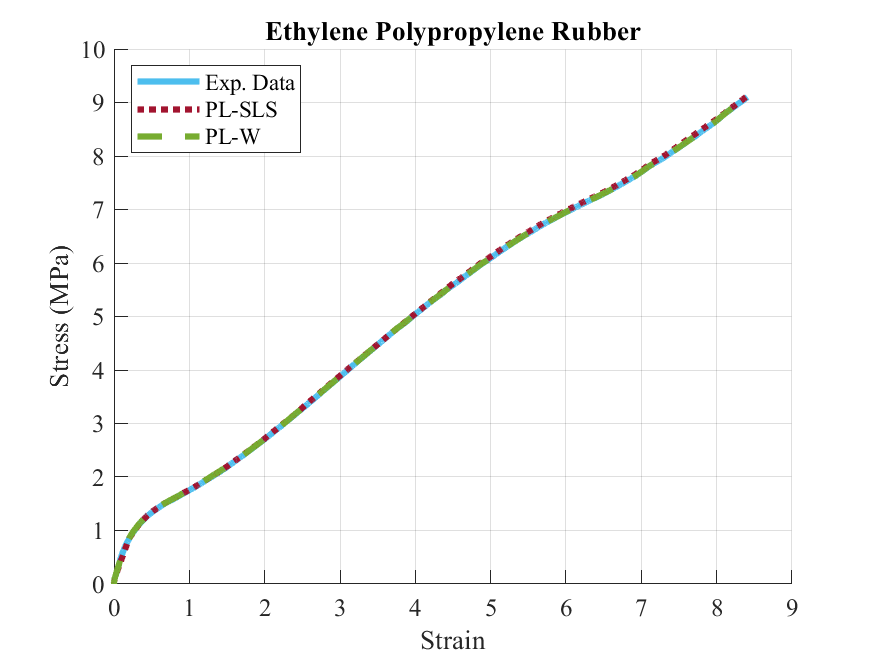
\includegraphics[width=\textwidth]{EPR_PLModelsBestFit.png}
		\caption{}
		\label{fig:BestFitEPR}
	\end{subfigure}
	\begin{subfigure}[b]{0.9\textwidth}
		\centering
		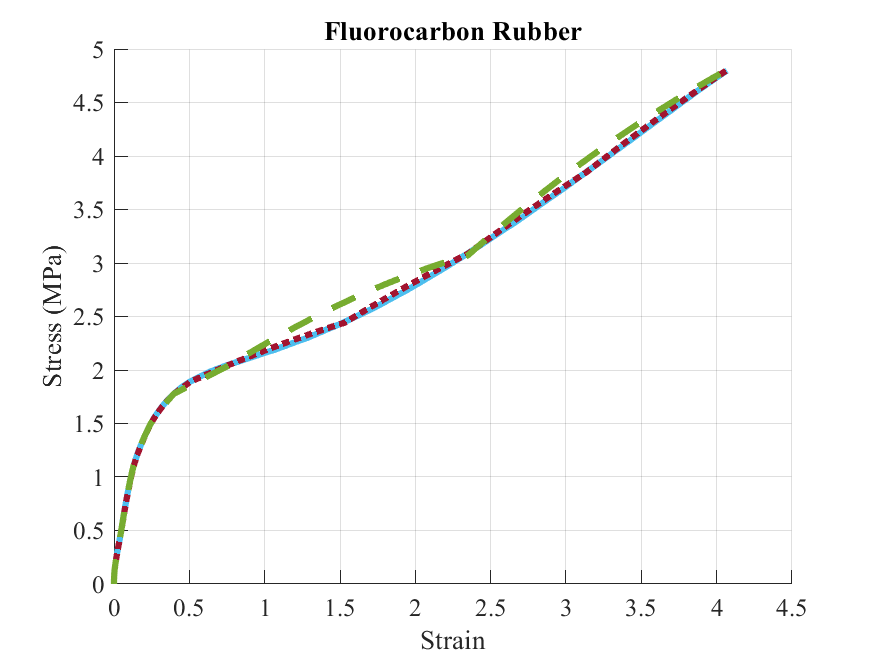
\includegraphics[width=\textwidth]{FR_PLModelsBestFit.png}
		\caption{}
		\label{fig:BestFitFR}
	\end{subfigure}
	\caption{Best fit for the PL-SLS and PL-Wiechert models on the stress-strain curve of (a) EPR material (b) FR material. The parameters required for this fit can be found in \Cref{tbl:PLModelsPerformance}. }
	\label{fig:BestFitEPR_FR}
\end{figure}

\begin{figure}[H]
	\centering
	\begin{subfigure}[b]{0.9\textwidth}
		\centering
		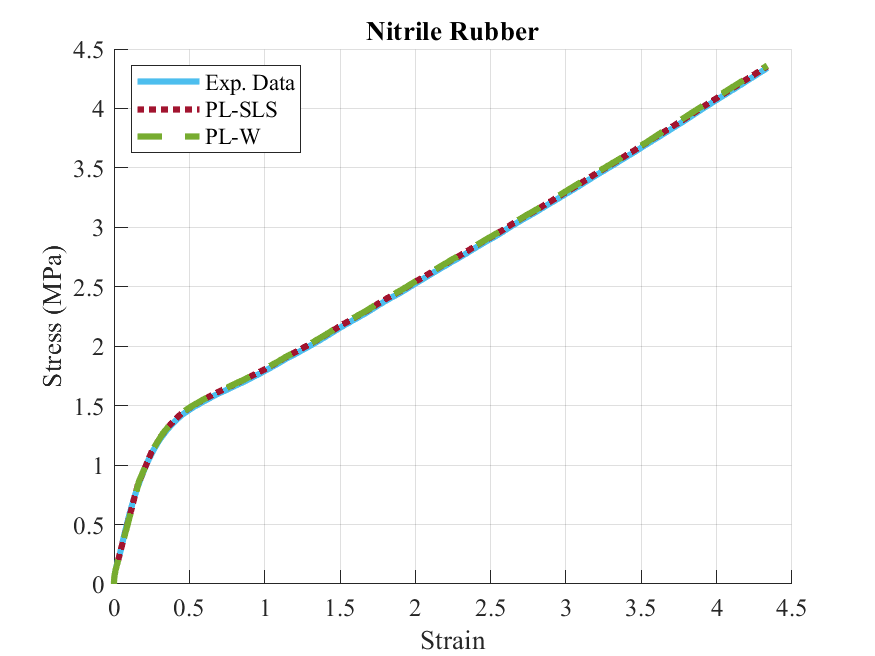
\includegraphics[width=\textwidth]{NR_PLModelsBestFit.png}
		\caption{}
		\label{fig:BestFitNR}
	\end{subfigure}
	\begin{subfigure}[b]{0.9\textwidth}
		\centering
		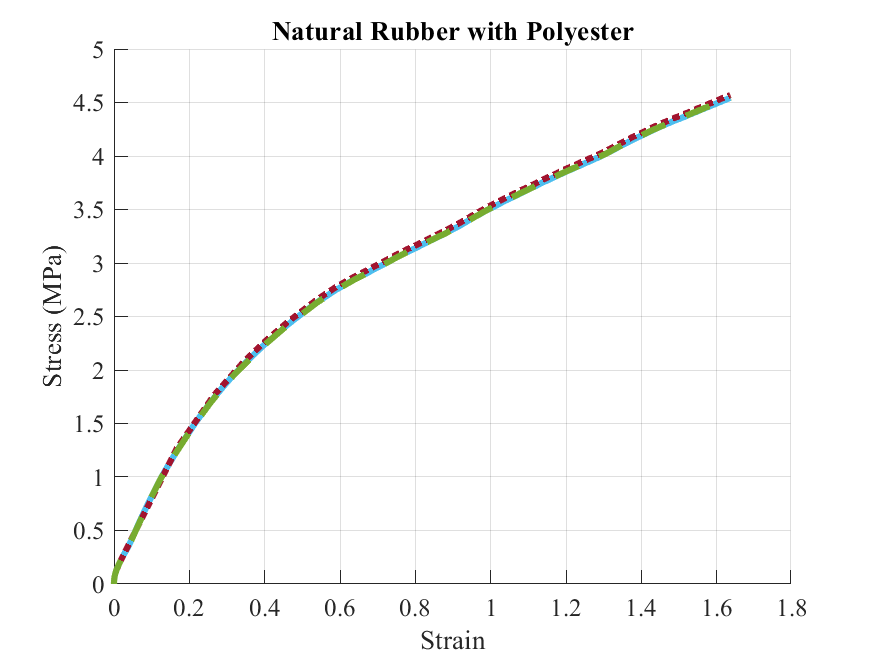
\includegraphics[width=\textwidth]{NatR_PLModelsBestFit.png}
		\caption{}
		\label{fig:BestFitNatR}
	\end{subfigure}
	\caption{Best fit for the PL-SLS and PL-Wiechert models on the stress-strain curve of (a) NR material (b) NatPolR material. The parameters required for this fit can be found in \Cref{tbl:PLModelsPerformance}. }
	\label{fig:BestFitNR_NatR}
\end{figure}

\begin{figure}[H]
	\centering
	\begin{subfigure}[b]{0.9\textwidth}
		\centering
		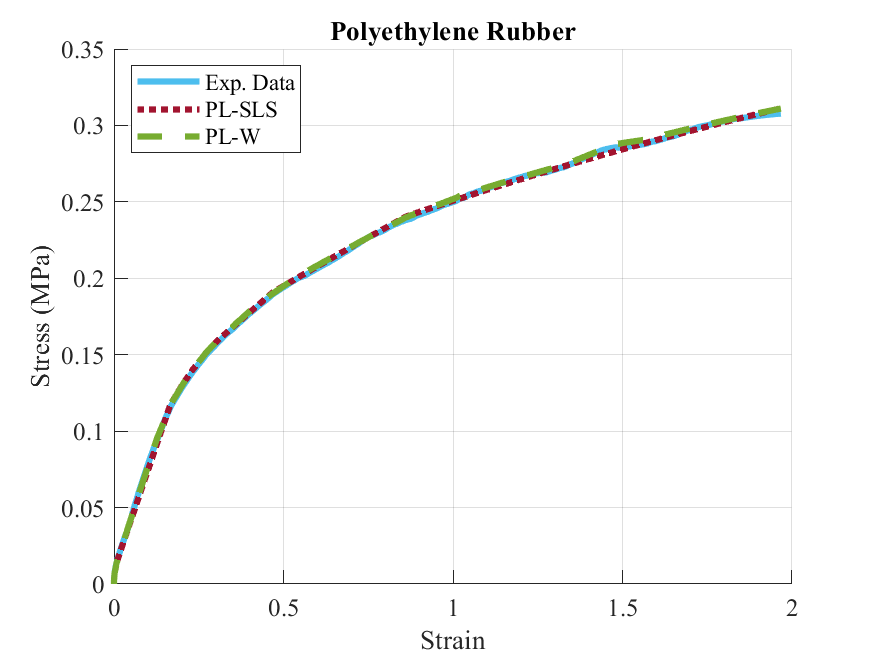
\includegraphics[width=\textwidth]{PR_PLModelsBestFit.png}
		\caption{}
		\label{fig:BestFitPR}
	\end{subfigure}
	\begin{subfigure}[b]{0.9\textwidth}
		\centering
		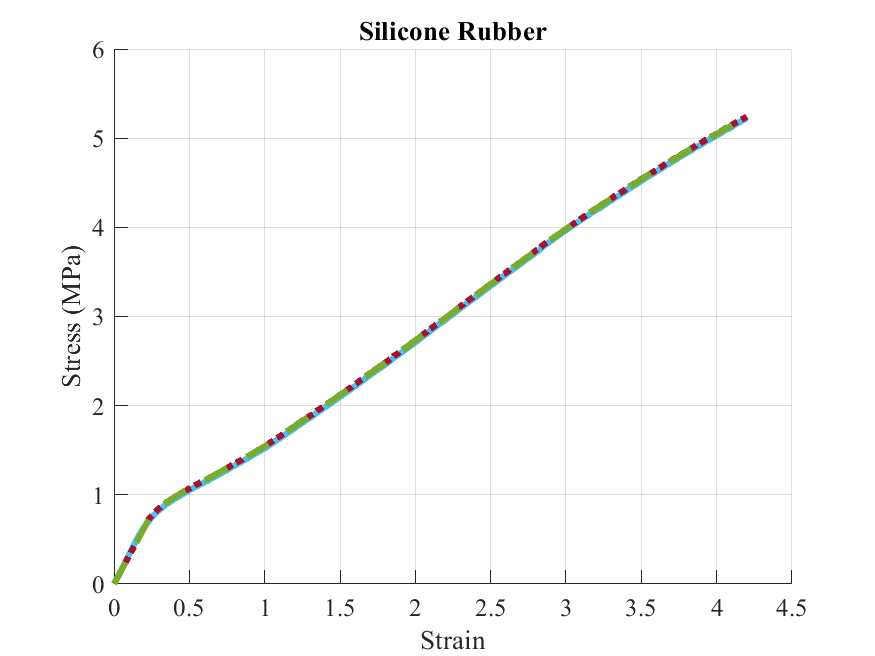
\includegraphics[width=\textwidth]{SR_PLModelsBestFit.png}
		\caption{}
		\label{fig:BestFitSR}
	\end{subfigure}
	\caption{Best fit for the PL-SLS and PL-Wiechert models on the stress-strain curve of (a) PR material (b) SR material. The parameters required for this fit can be found in \Cref{tbl:PLModelsPerformance}.}
	\label{fig:BestFitPR_SR}
\end{figure}

\begin{figure}[H]
	\centering
	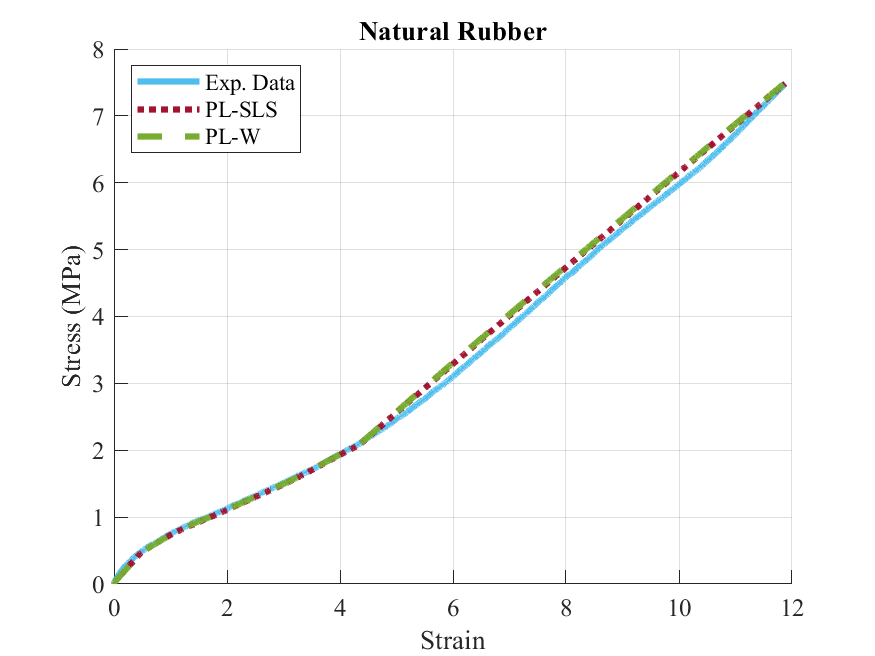
\includegraphics[width=0.9\textwidth]{Nat100R_PLModelsBestFit.png}
	\caption{Best fit for the PL-SLS and PL-Wiechert models on the stress-strain curve of NatR material. The parameters required for this fit can be found in \Cref{tbl:PLModelsPerformance}.}
	\label{fig:BestFitNat100R}
\end{figure}


\subsection{Analysis on the velocity-dependent stress response} \label{VelocityAnalysis}

In previous sections, the performance of both the PL-SLS model and PL-Wiechert model is found ot be very similar for all the studied soft materials. The main difference between the models is the required complexity to achieve said accuracy. In this section, the capability of both models to account for the velocity-dependent stress response of the soft material is analyzed. The result of this analyses can provide a better way to determine whcih of the developed models is the best choice for each soft material. Moreover, the PL-SLS and the PL-Wiechert models are inspired on the work of Austin et al. where a similar model, the Std. Lin. SDS model was developed \cite{austin2015control}. Similarly, the capabilities of the Std. Lin. SDS model of accurately describing the velocity-dependent stress response of the soft material used was not assessed due to hardware limitations. Due to this, the latter property is investigated in this section. 

The PL-SLS model and the PL-Wiechert model analyzed so far are the result of applying the PL method to the stress-train curve of the soft materials obtained from the tensile strength test. The strain rate used in these tests varies from one material to the other. Almost in all cases the 500 mm/min strain rate is used for the fitting process. The only exception is the SR material where a the strain rate of 50 mm/min is used instead. The dataset of the studied soft materials contains up to three different strain rates per material, as described in \Cref{tbl:tensile_tests}. 

The strain-dependent stiffness $k^*$ is the result of fitting the PL method to the SLS and the Wiechert models. This parameter is the linearized version of the equilibrium spring stiffness contained in both LVMs. The obtained $k^*$ for each soft material is specific to one strain rate. In the following analysis, the strain-dependent stiffness of the equilibrium spring $k^*$ has a major role. Therefore, the analysis in this section investigates the performance of the PL-SLS model and the PL-Wiechert model when using the obtained $k^*$ under different strain rates.

In \Cref{SegmentAnalysis,ModelfitAnalysis}, the NRMSE and the number of strain segments are used to measure the performance of both the Pl-SLS and the PL-Wiechert models. There is a clear trade-off between the achieved accuracy and the required model complexity. In these analyses, the case for which the NRMSE value is the smallest do not reflect the best fit for the task of accounting for the velocity-dependent stress response of the soft materials. In fact, this can cause the fitted model to only perform well for a specific set of data, or in this case, a specific strain rate. Therefore, the main focus of the analysis performed in this section is to obtain the number of strain segments, i.e. a $k^*$, for each material that allows the PL-SLS model and the PL-Wiechert model to predict the stress-train curve of the materials for different strain rates. The latter also assesses the generalization capabilities of the developed models.

The analysis performed in here is an extension of the one performed in \Cref{SegmentAnalysis}. In here, the prediction of the models for the strain rates of 50 min/mm, 250 min/mm, and 500 min/mm is obtained. The same range of tolerance values is used in here. Similarly, the NRMSE is used to measure the models accuracy. The results are illustrated in \Cref{fig:FitAllEPR_FR,fig:FitAllNR_NatR,fig:FitAllPR_SR,fig:FitAllNat100R}. In addition to this, the generalization error of both models is calculated as the mean NRMSE value along all strain rates for a single tolerance value, as follows:


\begin{equation}
	\label{eqGE}
	GE = \frac{1}{N}\sum_{j=1}^{N} NRMSE_j
\end{equation}

\noindent where $N$ is the total number of strain rates cases, up to 3, and $j$ is the individual strain rate case.


\begin{figure}[H]
	\centering
	\begin{subfigure}[b]{0.9\textwidth}
		\centering
		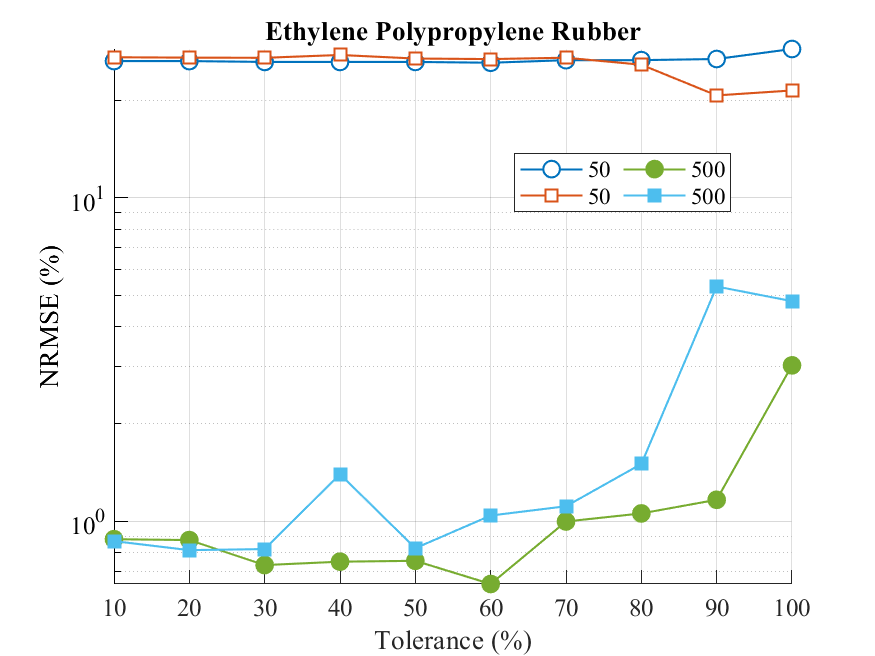
\includegraphics[width=\textwidth]{EPR_PLMethodFitAll.png}
		\caption{}
		\label{fig:FitAllEPR}
	\end{subfigure}
	\begin{subfigure}[b]{0.9\textwidth}
		\centering
		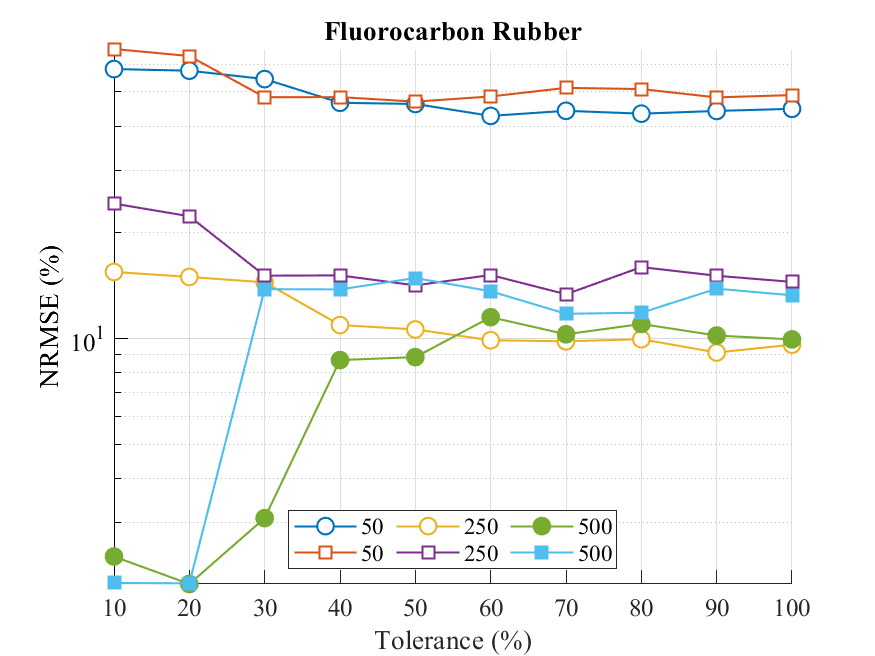
\includegraphics[width=\textwidth]{FR_PLMethodFitAll.png}
		\caption{}
		\label{fig:FitAllFR}
	\end{subfigure}
	\caption{Prediction of the PL-SLS (circles) and the PL-Wiechert (squares) model under different strain rates for the (a) EPR material (b) FR material. Strain rates are in millimeters per minute. Filled markers indicate the strain rate used to extract the strain dependent stiffness $k^*$. }
	\label{fig:FitAllEPR_FR}
\end{figure}

\begin{figure}[H]
	\centering
	\begin{subfigure}[b]{0.9\textwidth}
		\centering
		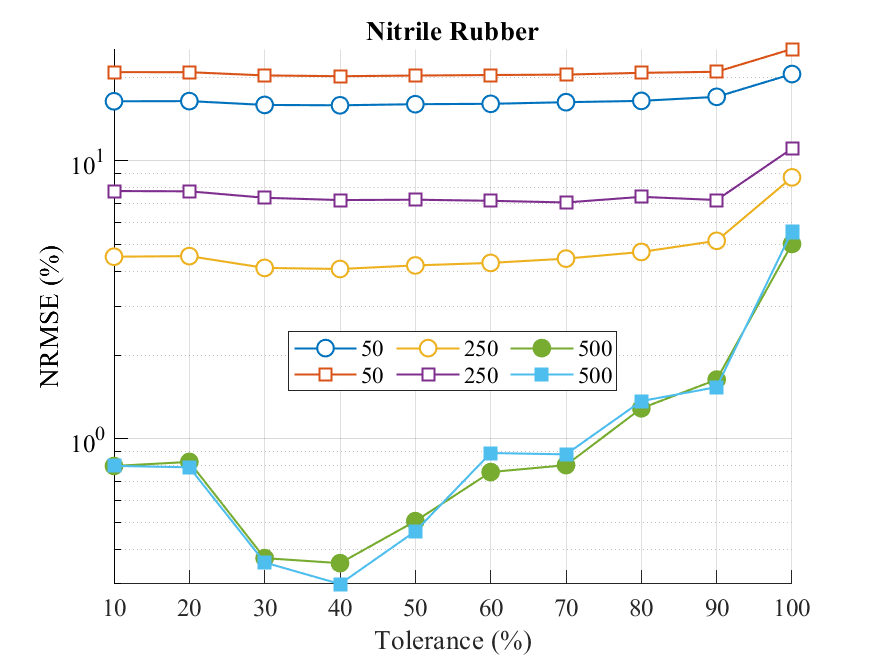
\includegraphics[width=\textwidth]{NR_PLMethodFitAll.png}
		\caption{}
		\label{fig:FitAllNR}
	\end{subfigure}
	\begin{subfigure}[b]{0.9\textwidth}
		\centering
		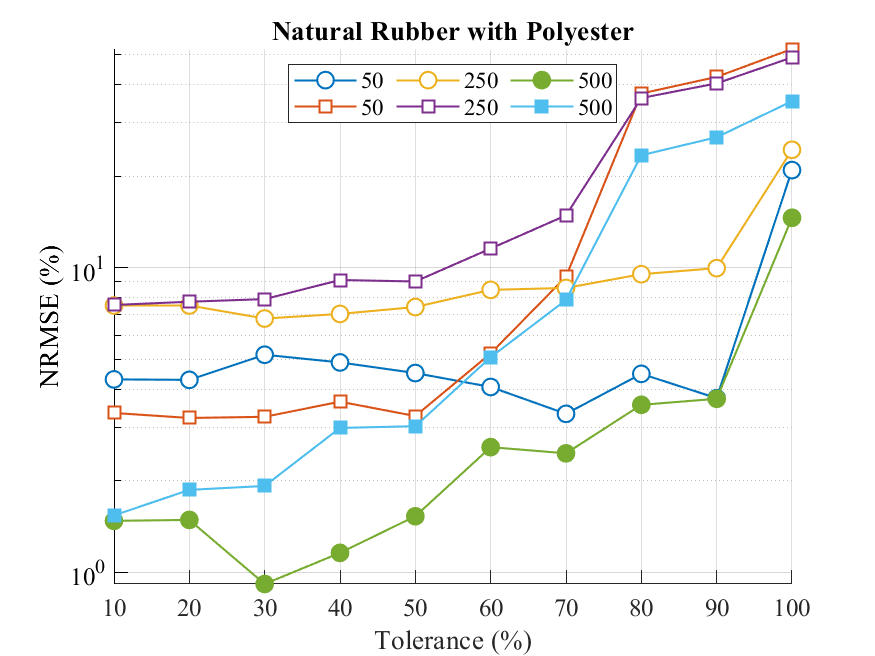
\includegraphics[width=\textwidth]{NatR_PLMethodFitAll.png}
		\caption{}
		\label{fig:FitAllNatR}
	\end{subfigure}
	\caption{Prediction of the PL-SLS (circles) and the PL-Wiechert (squares) model under different strain rates for the (a) NR material (b) NatR material. Strain rates are in millimeters per minute. Filled markers indicate the strain rate used to extract the strain dependent stiffness $k^*$. }
	\label{fig:FitAllNR_NatR}
\end{figure}

\begin{figure}[H]
	\centering
	\begin{subfigure}[b]{0.9\textwidth}
		\centering
		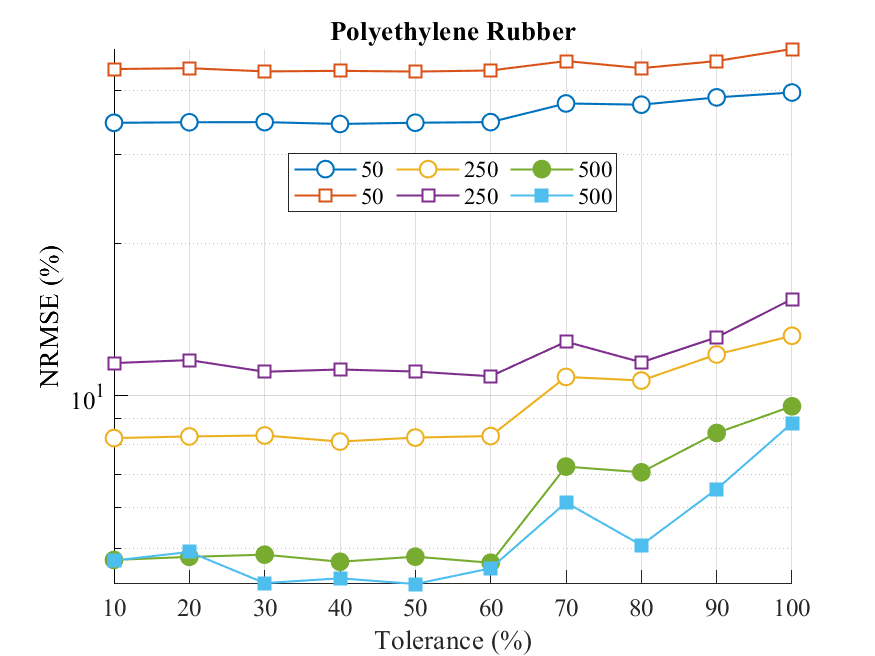
\includegraphics[width=\textwidth]{PR_PLMethodFitAll.png}
		\caption{}
		\label{fig:FitAllPR}
	\end{subfigure}
	\begin{subfigure}[b]{0.9\textwidth}
		\centering
		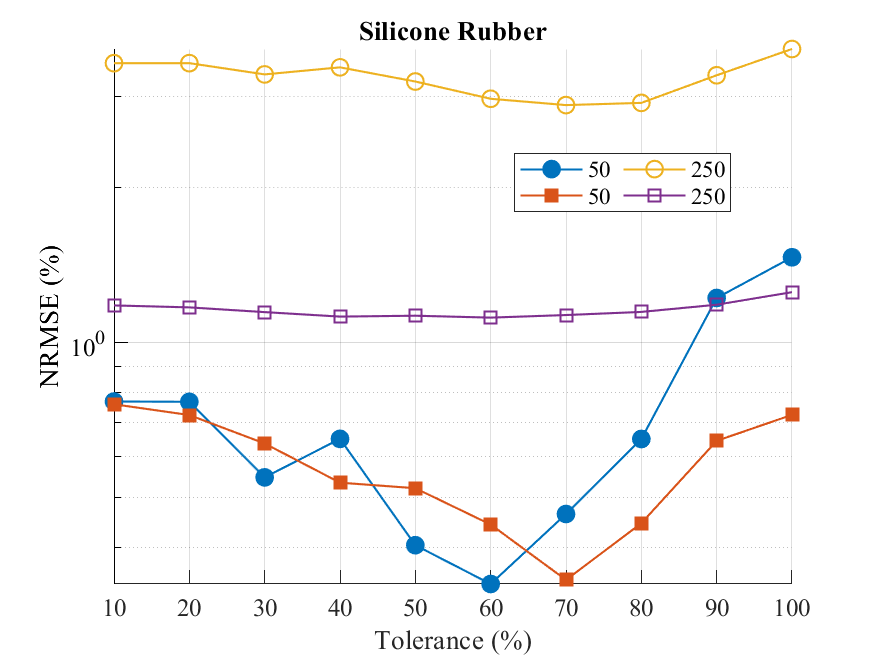
\includegraphics[width=\textwidth]{SR_PLMethodFitAll.png}
		\caption{}
		\label{fig:FitAllSR}
	\end{subfigure}
	\caption{Prediction of the PL-SLS (circles) and the PL-Wiechert (squares) model under different strain rates for the (a) PR material (b) SR material. Strain rates are in millimeters per minute. Filled markers indicate the strain rate used to extract the strain dependent stiffness $k^*$.}
	\label{fig:FitAllPR_SR}
\end{figure}

\begin{figure}[H]
	\centering
	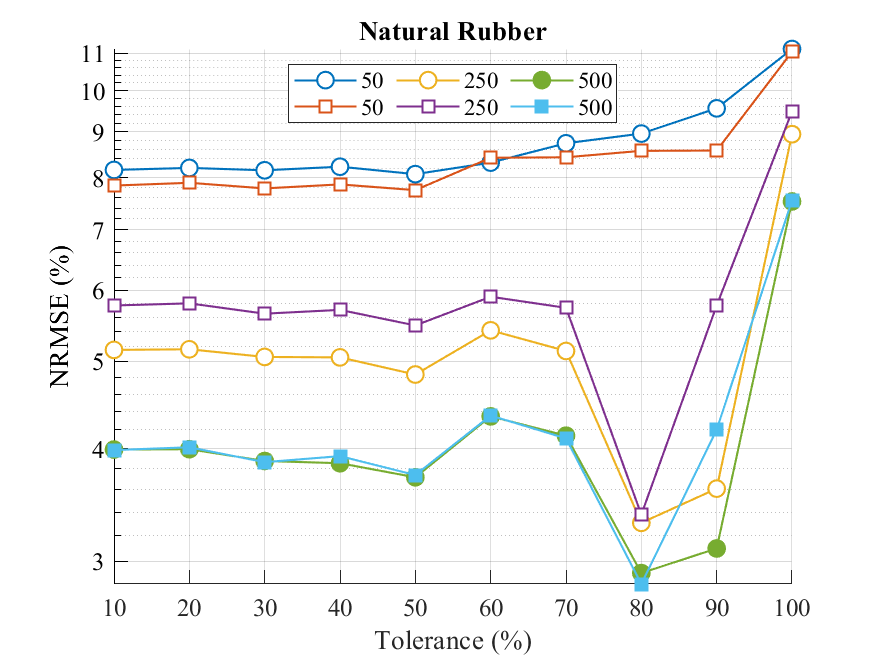
\includegraphics[width=0.9\textwidth]{Nat100R_PLMethodFitAll.png}
	\caption{Prediction of the PL-SLS (circles) and the PL-Wiechert (squares) model under different strain rates for the NatR material. Strain rates are in millimeters per minute. Filled markers indicate the strain rate used to extract the strain dependent stiffness $k^*$.}
	\label{fig:FitAllNat100R}
\end{figure}

From previous figures, an interesting tendency is revealed. For the cases in which the strain rate of 500 mm/min is used to obtain the strain dependent stiffness $k^*$, the accuracy of both models decreases in proportion to the difference between the predicted strain rate and the strain rate used for fitting. In contrast, for the cases in which the strain rate of 50 mm/min is used for fitting, i.e. for the SR material, the accuracy of both models behaves differently (\Cref{fig:FitAllSR}). In this scenario, the PL-Wiechert model performs better than the PL-SLS model. The latter finding could suggest that using a slower strain rate for extracting the $k^*$ delivers better results. Although, there are some variables to take into account before jumping to any conclusion, such as the type of material, and overall complexity of the model used. Nonetheless, considering the velocity-dependency stress response of the elements on the Maxwell branches for both models, using a slower strain rate has the potential to better isolate the stress response of the equilibrium spring $k_e$. In other words, this approach has the potential to improve the PL method fitting process for the PL method fitting.

For almost all cases, the PL-SLS achieve smaller NRMSE values than the PL-Wiechert model, with the exception of the SR and NatR materials \Cref{fig:FitAllSR,fig:FitAllNat100R}. Nonetheless, the overall performance of each model is better assessed using the generalization error, $GE$. Therefore, the tolerance value which yielded the smallest $GE$ is calculated and reported in \Cref{tbl:GenError}.

\begin{table*}[htbp!]
	\centering
	\caption{Best generalization error of the PL-SLS (1) and the PL-Wiechert (2) models.}
	\label{tbl:GenError}
	\begin{tabular}{llccccccc} \toprule
		Model 					& Parameters 		& EPR	& FR 	& NatPolR & NR & PR & SR & NatR \\
		\hline
		\multirow{2}{*}{1}  & Gen. Error (\%)		& 13.04	& 3.03 	& 2.27 	& 1.36 & 2.70 & 1.44 & 1.10 \\
		& Tolerance (\%)							& 60	& 90 	& 30 	& 40 	& 40 & 70 & 80 \\
		\hline 
		\multirow{2}{*}{2}  & Gen. Error (\%)		& 10.34	& 4.44 	& 2.51 	& 2.36 & 3.64 & 0.55 & 1.12\\		
		& Tolerance	(\%)							& 90	& 70 	& 10 	& 70 	& 60 & 60 & 80 \\		
		\bottomrule
	\end{tabular}
\end{table*}

The obtained best case generalization errors are in line with the best case NRMSE values reported in \Cref{tbl:PLModelsPerformance}. In here, the PL-SLS model outperforms the PL-Wiechert model for all but two materials, the EPR and the SR materials. For specific case of the SR material, the PL-Wiechert model performs much better than the PL-SLS model. The reason for this is the small value of strain rate used for fitting the PL method to the stress-strain curve of the SR material. In all cases, both models achieve a $GE$ value smaller then 5\% which indicates that the models are capable of accounting for the velocity-dependent stress response of the studied soft materials. The exception to this is the EPR material which delivered a very large $GE$ value in comparison to the other materials. The larger $GE$ value in here can be attributed to the absent of a dataset for the strain rate of 250 mm/min. This create a larger gap between the prediction at 50 mm/min and the prediction at 500 mm/min, which is reflected when calculating the mean NRMSE along all strain rates, i.e. the $GE$ described in \Cref{eqGE}. On top of this, the potential disadvantage of using the strain rate of 500/min can also be influencing the performance of both models for this particular soft material. Lastly. the models developed in here achieved a higher performance in comparison to the Std. Lin. SDS model documented in the literature. The reported relative RMSE value for the Std. Lin. SDS model when is of 13.6\%. The conditions in which the latter performance is achieved are comparable to the conditions in \Cref{ModelfitAnalysis}, where the reported NRMSE values for both models are in the range of 0.34 to 4.67\% (\Cref{tbl:PLModelsPerformance}). Similarly, the generalization error $GE$ obtained in this section further validate the much better performance achieved by the PL-SLS and the PL-Wiechert models.

Summarizing, in this section the capabilities of the PL-SLS and the PL-Wiechert model of accounting for the velocity-dependent stress response of the soft materials is assessed. This is measured using the generalization error, $GE$, described in \Cref{eqGE}. The results indicate that both models are capable of predicting the stress response of the soft materials under different strain rates with reasonable accuracy. In other words, they are capable of accounting for the velocity-dependent stress response of the soft materials. The only exception to this conclusion is the EPR material, where a larger $GE$ value was obtained. The potential causes of this isolated case are the larger gap between the strain rate used for the fitting process and the predicted strain rate, and the potential limitations of using 500 mm/min instead of 50mm/min as the strain rate for the fitting process. Using the strain rate of 50 mm/min is found to be beneficial for the performance of both models as observed in the results for the SR material.

\section{Summary}

In this chapter, the development process of the PL-SLS and the Pl-Wiechert is described. The fitting process of both models is very similar, as described in \Cref{fig:FCFittingProcess}. The main differences between the developed models in here and the Std. Lin. SDS model found in the literature \cite{austin2015control} are the following optimizations: 

\begin{itemize}
	\item Transform the constitutive differential equations of both models into their finite differences form. This allowed the PL method to be easily implemented to both models.
	\item Logarithmic time collocation approach to extract the values of $k_j$ and $\tau_j$ from the stress relaxation curve.
	\item Removal of the stress response of the components in the Maxwell branches.
	\item Propose a tolerance criteria based on the variation of the stress-strain curve to determine the number of strain segments to be fitted.
\end{itemize}

In addition to the latter differences, several aspects of the piecewise linearization method are investigated in this section. Firstly, the relationship between the complexity and the accuracy of the PL method is described in \Cref{SegmentAnalysis}. The latter is achieved due to the proposed tolerance criteria which is based on the slope variation of the stress-strain curve. The obtained results, illustrated in \Cref{fig:SegmentsEPR_FR,fig:SegmentsNR_NatR,fig:SegmentsPR_SR,fig:SegmentsNat100R}, describe the relationship between the required complexity and the achieved accuracy for both the PL-SLS and the PL-Wiechert model. Both models behave different depending on the soft material. The latter can be used to categorize the studied soft materials in highly elastic, viscoelastic, and highly viscous. The PL-SLS model performs better for soft materials in the highly elastic category, wheres the PL-Wiechert performs better for soft materials in the viscoelastic and highly viscous categories. The latter is in line with the fundamentals behind each model where the PL-Wiechert model has many Maxwell branches to describe many time constants of the material, i.e. many viscous constants. 

Secondly, in \Cref{ModelfitAnalysis} the performance of both developed models is investigated. The obtained results are compiled in \Cref{tbl:PLModelsPerformance}, where the PL-SLS model is suggested as the best choice for most cases. The additional complexity of using the PL-Wiechert model does not justify the performance improvement. Nonetheless, in this analysis the models are only assessed in their capabilities of fitting the stress-strain curve for a single strain rate. This conclusion changes when considering the models capability of accounting for different strain rates.

Thirdly, the analysis described in \Cref{VelocityAnalysis} is focused on assessing the capabilities of the developed models of accounting for the velocity-dependent stress response of the soft materials. In other word, the generalization capabilities of the developed models are assessed. In here, the obtained strain dependent stiffness $k^*$ is used to predict the stress-strain curve of the soft materials under different strain rates. Up to three different values of strain rates are evaluated: 50, 250, and 500 mm/min. The performance of the models are assessed using the generalization error $GE$ described in \Cref{eqGE}. In general, the PL-SLS model outperforms the PL-Wiechert model for all but two materials, the EPR and the SR materials. For the specific case of the SR material, the PL-Wiechert model performs much better than the PL-SLS model. The differences in performance can be cause by the strain rate used for the extraction of the strain dependent stiffness $k^*$. The results are compiled in \Cref{tbl:GenError}. In all cases, both models achieve a $GE$ value smaller then 5\% which prove the capability of the models to account for the velocity-dependent stress response of soft materials. The only isolated case in which the achieved $GE$ is higher than 5\% is for the EPR material. The potential cause for this is the strain rate used for fitting process of the PL method. This further validate the hypothesis that using a small values of the strain rate is beneficial for the fitting process of the PL method.

Finally, the PL-SLS and the PL-wiechert models achieved a higher prediction accuracy in comparison to the Std. Lin. SDS model documented in the literature. The reported relative RMSE value for the Std. Lin. SDS model when is of 13.6\%. The conditions in which the latter performance is achieved are comparable to the conditions in \Cref{ModelfitAnalysis}, where the reported NRMSE values for both models are in the range of 0.34 to 4.67\% (\Cref{tbl:PLModelsPerformance}). Similarly, the prediction accuracy of the models developed in here when accounting for different strain rates, reported as $GE$ values in \Cref{tbl:GenError} in \Cref{VelocityAnalysis}, further validate the much better performance achieved by the PL-SLS and the PL-Wiechert models in comparison to their predecessor the Std. Lin. SDS model. The performance of the Std. Lin. SDS model under this scenario was not assessed in the literature. The superiority of the PL-SLS and the PL-Wiechert models is due to the many optimizations performed to the PL method fitting process.

%The experimental data obtained from the stress relaxation tests of six soft materials is used to describe the parameters of two mathematical models, the SLS and the Wiechert model. Both models were fit into the stress relaxation curve to extract their parameters. The fitting process for the SLS model is straight forward and the simplicity of the model yielded in a large RMSE. In contrast, the Wiechert model was fitted using a time collocation technique which yielded in a system of equations required to be solved to obtain all the model parameters. In addition to this, an optimization algorithm is implemented to obtain the right amount of Maxwell branches required to minimize the RMSE. The optimal number of branches varies from one material to the other in the range of $j=[8,10]$. The stress response of the optimal number of Maxwell branches is subtracted from the tensile strength test data. This step allows the piecewise linearization to better approximate the strain-dependent stiffness of the equilibrium spring. Due to the lack of explicit information regarding the PL method implementation \cite{austin2015control}, an algorithm to locate the strain segments for the PL method using the variation of the slope of the stress-strain curve as the selection criteria, is developed. The relationship between the previous tolerance with the achievable NRMSE and the number of strain segments is obtained (\Cref{fig:SegmentsAll}). These set of charts have the potential to be used as design guidelines when using the reported soft materials in robotic applications, since they highlight the trade-off between the achievable accuracy and the computational cost. The process of implementing the PL method into the linear viscoelastic models yielded the PL-Wiechert and PL-SLS models. These models are presented in the form of finite difference equations to evaluate their stress response. The results demonstrates the great accuracy of the PL-SLS model in describing the stress-strain curve of six soft materials, in comparison to the PL-wiechert model. The PL-method turned out to be incompatible with the Wiechert model. The latter is due to an essential difference between \Cref{eq6} and \Cref{eq7}. In the latter equation, $k_i^*$ interacts with the strain and the strain rate whereas in the former, $k_i^*$ only interacts with the strain. This lack of interaction allows the abrupt step changes caused by the Heaviside function to disturb the PL-Wiechert model response. The analysis performed up to this point included six out of the seven soft materials. The material missing is the Natural Rubber.

%The developed PL-SLS model, an optimized version of the Std. Lin. SDS model, was identified as the best candidate for the prediction of the nonlinear and strain-dependent stress response of the studied soft materials. In addition to this, the capabilities of the PL-SLS model to account for velocity-dependent stress responses was assessed. This analysis was not available in the reviewed literature. The analysis, which included all of the seven soft materials, yielded very interesting findings. On the one hand, the PL-SLS model is able to generalize well the stress-stain curves of the NatPolR, SR, and NatR materials, for up to three different strain rates. On the other hand, the PL-SLS model performed very poorly for the remaining materials. The poor performance of the PL-SLS model is directly related to the fact that the model only accounts for one time relaxation constant. In other words, the PL-SLS model is able to generalize well the stress response under different strain rate of viscoelastic soft materials with more dominant elastic properties. Therefore, the model capabilities to account for velocity-dependent (time-dependent) stress responses is poor. Lastly, due to the latter findings, an alternative modelling tool is investigated in the following chapter.